\documentclass{ctexbook}
\usepackage{graphicx}
\usepackage{fancyhdr}
\usepackage[top=2cm,bottom=2cm,left=2cm,right=1cm]{geometry}

\usepackage{mathtools}
\usepackage{amsthm}
\usepackage{cases}
\usepackage{bm}
\usepackage{algorithm}
\usepackage{algorithmic}
\usepackage{url}
\usepackage{subfigure}
\usepackage{xcolor}
\usepackage{textcomp}
\usepackage{listings}
\usepackage{animate}
\usepackage{amssymb}%\because����
\usepackage{fancyhdr}
\graphicspath{{figures/},{figures/_1perception/},{figures/_2SVD/},{figures/_3naivebayes/},{figures/_4pagerank/},{figures/_1perception/perception1/}}

\newtheoremstyle{mythm}{1.5ex plus 1ex minus .2ex}{1.5ex plus 1ex minus .2ex}{}{\parindent}{\bfseries}{}{1em}{} \theoremstyle{mythm}
\newtheorem{thm}{����~}
\newtheorem{lem}{����~}
\newtheorem{prop}{����~}
\newtheorem{cor}{����~}
\newtheorem{defn}{����~}
\newtheorem{conj}{����~}
\newtheorem{exmp}{��~}
\newtheorem{rem}{ע~}

\makeatletter % `@' now normal "letter"
\@addtoreset{equation}{section}
\makeatother  % `@' is restored as "non-letter"
\renewcommand\theequation{\oldstylenums{\thesection}.\oldstylenums{\arabic{equation}}}
\definecolor{mygreen}{rgb}{0,0.6,0}
\definecolor{mygray}{rgb}{0.5,0.5,0.5}
\definecolor{mymauve}{rgb}{0.58,0,0.82}
\lstset{ %
  backgroundcolor=\color{white},   % choose the background color; you must add \usepackage{color} or \usepackage{xcolor}
  basicstyle=\footnotesize,        % the size of the fonts that are used for the code
  breakatwhitespace=false,         % sets if automatic breaks should only happen at whitespace
  breaklines=true,                 % sets automatic line breaking
  captionpos=bl,                    % sets the caption-position to bottom
  commentstyle=\color{mygreen},    % comment style
  deletekeywords={...},            % if you want to delete keywords from the given language
  escapeinside={\%*}{*)},          % if you want to add LaTeX within your code
  extendedchars=true,              % lets you use non-ASCII characters; for 8-bits encodings only, does not work with UTF-8
  frame=single,                    % adds a frame around the code
  keepspaces=true,                 % keeps spaces in text, useful for keeping indentation of code (possibly needs columns=flexible)
  keywordstyle=\color{blue},       % keyword style
  %language=Python,                 % the language of the code
  morekeywords={*,...},            % if you want to add more keywords to the set
  numbers=left,                    % where to put the line-numbers; possible values are (none, left, right)
  numbersep=5pt,                   % how far the line-numbers are from the code
  numberstyle=\tiny\color{mygray}, % the style that is used for the line-numbers
  rulecolor=\color{black},         % if not set, the frame-color may be changed on line-breaks within not-black text (e.g. comments (green here))
  showspaces=false,                % show spaces everywhere adding particular underscores; it overrides 'showstringspaces'
  showstringspaces=false,          % underline spaces within strings only
  showtabs=false,                  % show tabs within strings adding particular underscores
  stepnumber=1,                    % the step between two line-numbers. If it's 1, each line will be numbered
  stringstyle=\color{orange},     % string literal style
  tabsize=2,                       % sets default tabsize to 2 spaces
}



\begin{document}

\begin{titlepage}
\setcounter{page}{1}
\newcommand{\HRule}{\rule{\linewidth}{0.5mm}}
\begin{center}

\includegraphics[width=0.45\textwidth]{logobupt.jpg}\\[0.5cm]
\textsc{\LARGE Beijing University of Posts and Telecommunications}\\[1.5cm]
\HRule \\[0.2cm]
{ \huge \bfseries ������ѧϰ���γ��ܽ�}\\[-0.2cm]
\HRule \\[1.5cm]
\begin{table}[h]
  \centering
  \large  %���ڵ������С
  \begin{tabular}{cl}
    ����:\quad& ������\\
    ѧԺ:\quad& ���缼���о�Ժ\\
    ѧ��:\quad& 2014111469\\
    �ڿν�ʦ:\quad&�ž�ƽ����\\
  \end{tabular}
\end{table}
{\large 2015��1��5��}
\end{center}

\end{titlepage}
\frontmatter
\tableofcontents
\mainmatter
\pagestyle{fancy}
\fancyhf{}
\fancyhead[RE]{\normalfont\small\rmfamily\nouppercase{\leftmark}}
\fancyhead[LO]{\normalfont\small\rmfamily\nouppercase{\rightmark}}
\fancyhead[LE,RO]{\thepage}
\fancyfoot[LE,LO]{\small\normalfont ������ѧϰ����ĩ�ܽ�~By~������}
\fancyfoot[RE,RO]{\textsf{\small \color{blue} http://blog.csdn.net/u012176591}}

\chapter{���}
\section{�½ڼ��}
��һ�½����˸�֪��ģ�͵���ѧԭ����ģ���Ƶ����㷨��������һ��Pythonʵ�ֵ����ӡ���֪��ģ����������ģ�ͺ�֧��������ģ�͵Ļ������ڶ��½����������б�ģ��(LDA)������ֵ�ֽ�(SVD)�����ɷַ���ģ��(PCA)��������ģ��������������Ԥ�����Ľ�ά���̡������½��������ر�Ҷ˹ģ�ͣ�����һ������ģ�ͣ�����ģ�ͼ򵥡�Ч���������������ı�����ȵȡ������½�������ҳ����(PageRank)ģ�͵���ѧԭ����
\section{������Դ}
���������ݣ���֪��ģ�ͣ�LDA��SVD��PCAģ�ͣ����ر�Ҷ˹ģ�ͣ�PageRankģ�ͣ��ֱ������ڱ�ѧ������CSDN��д����ƪ���ͣ����ǵIJ������֡���ַ�ͷ���ʱ�����±���ʾ


\begin{table}[!ht]
  \centering
  \caption{��ƪ���͵IJ������֡���ַ�ͷ���ʱ���}
  \label{tab:xiangmuyuansu}
  \begin{tabular}{c|p{5cm}|c}
    \hline
    ����&��ַ&����ʱ��\\
    \hline
    LDA\_PCA\_SVD���� & \url{http://blog.csdn.net/u012176591/article/details/41923105} & 2014-12-14\\
    \hline
    ��֪������ & \url{http://blog.csdn.net/u012176591/article/details/41792857} & 2014-12-07\\
    \hline
    Naive Bayes���� & \url{http://blog.csdn.net/u012176591/article/details/41681907} & 2014-12-02\\
    \hline
    PageRank�������ѧ & \url{http://blog.csdn.net/u012176591/article/details/41597605} & 2014-11-29\\
    \hline
  \end{tabular}
\end{table}

�ҵ�CSDN���͵�������``����ɽׯ''��ȡ�����ұ��˵����֣���Ϊ``������־ͬ���ϵ��˷���ѧϰ�Ĺ���''����ַ\url{http://blog.csdn.net/u012176591/article}������ȥ��3�µ�4��֮�������Ʊ���ʱ���IJ��ͣ�����������ʼǵ���ʽд���͵ģ��������ۼ�188ƪ���ģ���Ȼ���Ƚϴ�ª���Ͼ���ֻ��һ���õĿ�ʼ�������ҵIJ��ͷ������Ѵ�80453�˴Ρ��������ҵIJ��͵Ľ�ͼ
\begin{figure}[!ht]
\centering
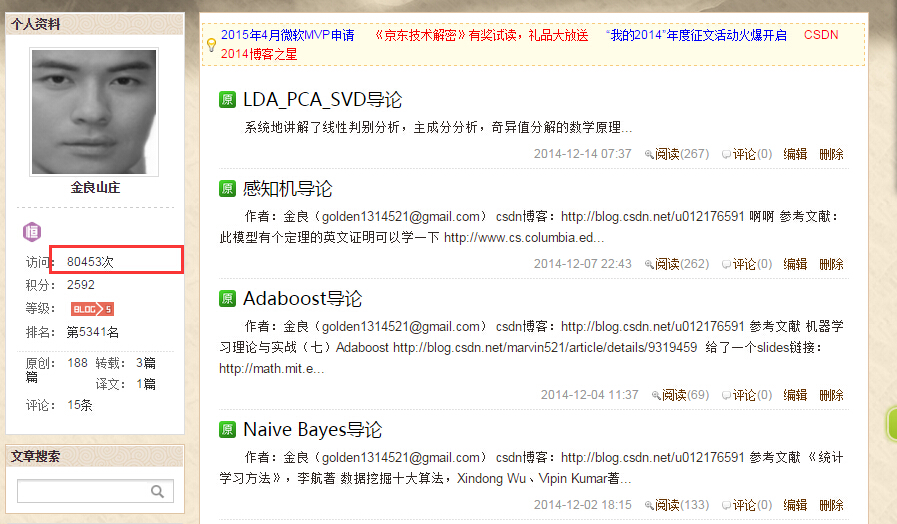
\includegraphics[width=0.85\textwidth]{blog.jpg}
\caption{�ҵ�CSDN����ʾ��ͼ}
\label{fig:hyperplane}
\end{figure} 



\newcommand{\button}[1]{\raisebox{-0.3ex}{\includegraphics[width=1.0em]{#1.jpg}}}

\chapter{��֪��ģ�ͽ���}
\section{��֪��Ҫ���������}
��֪��(perception)�ǵ�{\bf ���Կɷֶ�����ģ��}��������Ϊʵ�������������������ʵ��������ǩ��ȡ$+1$��$-1$ֵ����֪��ѧϰּ������ܹ���ѵ�����ݽ������Ի��ֵķ��볬ƽ�棬����ѵ�����ݱ��������Կɷ֣����Ը�֪�������ܹ��ҵ����н⡣�����ϣ��ڲ�ͬ�ij�ʼֵ��ѵ�������£���֪��ģ�Ϳ��Եõ����������н⡣{\bf ��֪��ģ����������(ANN) ��֧��������(SVM)�Ļ���}��
\begin{figure}[!ht]
\centering
\subfigure[ģ�Ϳ���]{
\label{fig:a}
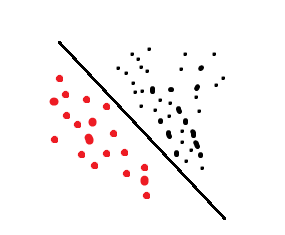
\includegraphics[width=0.4\textwidth,height=2.5in]{linear.png}}
\hspace{0.2in}
\subfigure[ģ�Ͳ�����]{
\label{fig:b}
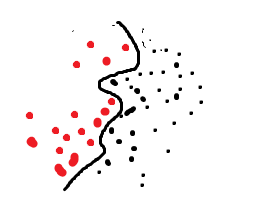
\includegraphics[width=0.4\textwidth,height=2.5in]{nonlinear.png}}

\caption{��֪��ģ�������Զ�����ģ�ͣ���ֻ���������Կɷֵ�����(image \ref{fig:a})���������������Բ��ɷֵ�����(image \ref{fig:b})����ѵ�����ݲ��ɷ�ʱ����֪��ģ��ѧϰ���̲���������������ᷢ����.}
\label{fig:todeal}
\end{figure}
\section{��֪��ģ��}
\begin{defn}\label{defn:perception}{\bf ��֪��ģ��\quad} ��������ռ�(�����ռ�)��$\chi \subseteq \mathcal{R}^{n}$������ռ���$mathcal{Y}=\{+1,-1\}$������$x\in \chi$��ʾʵ����������������Ӧ������ռ�(�����ռ�)��һ���㣻����$y\in \mathcal{Y}$ ��ʾʵ�������������ռ䵽����ռ�����º���
\begin{equation}
  f(\bm{x})=\mathrm{sign}(\bf{w}\cdot \bm{x}+b)
\end{equation}
��Ϊ��֪�������У�$\bm{w}$��$b$Ϊ��֪��ģ�Ͳ�����$\bm{w}\in \mathcal{R}^n$����Ȩֵ����(weight vector)��$b\in \mathcal{R}$����ƫ��(bias)��
\end{defn}

��֪��ģ�͵ļ���ռ��Ƕ����������ռ��е��������Է���ģ��(linear classification model)�����Է�����(linear classifier)������������$\{f|f(x)=\bf{w}\cdot \bm{x}+b\}$��

��֪���ļ��ν��ͣ����Է���
\begin{equation}
  \bf{w}\cdot \bm{x}+b=0
\end{equation}
��Ӧ�������ռ�$\mathcal{R}^{n}$�е�һ����ƽ��$S$,����$\bm{w}$�dz�ƽ��ķ�������$b$�dz�ƽ��Ľؾࡣ�����ƽ�潫�����ռ仮��Ϊ�����֣��ֱ�λ���������ֵĵ㣨����������������Ϊ���ࣨ��$\bf{w}\cdot \bm{x}+b>0\Rightarrow f(\bm{x})=1$���͸��ࣨ��$\bf{w}\cdot \bm{x}+b<0\Rightarrow f(\bm{x})=-1$������ˣ���ƽ��$S$��Ϊ���볬ƽ��(separating hyperplane)�� ��ͼ(\ref{fig:hyperplane})��ʾ���ֱ���Ϊ~\button{mycircle}~ ��~\button{mytriangle}~������ʵ�������볬ƽ�����ֿ����ֱ�λ�ڷ��볬ƽ���������ࡣ
\begin{figure}[!ht]
\centering
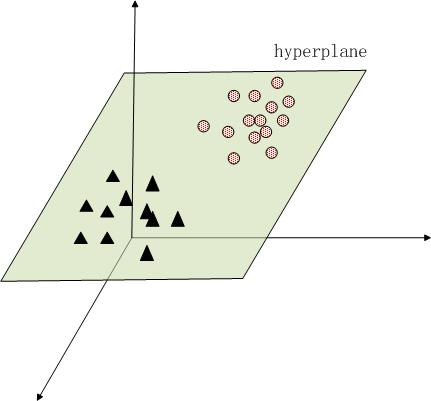
\includegraphics{hyperplane.jpg}
\caption{��ά�ռ�ķ��볬ƽ��ʾ��ͼ����ͬ��ǵ�����㼯�����볬ƽ��ֿ���}
\label{fig:hyperplane}
\end{figure}

��֪����ѧϰ�����Ǹ������ݼ�$T=\langle(\bm{x}_1,y_1),(\bm{x}_2,y_2),\cdots,(\bm{x}_N,y_N)\rangle$�����������ģ�Ͳ���$\bm{w}$��$b$�Ĺ��̡�����֪����ԤCE������ͨ��ѧϰ�õ��ĸ�֪��ģ�ͣ����µ�ʵ��$\bm{x}$ȷ��������ǩ$y$��
\section{��֪��ѧϰ����}
ȷ��ѧϰ���ԣ����Ƕ��壨���飩��ʧ����������ʧ������С����
\begin{defn}{\bf ��ʧ����\quad} ���賬ƽ��$S$�������㼯��Ϊ$M$����ô��֪������ʧ��������Ϊ
\begin{equation}
\label{equ:loss}
  \L(\bm{w},b)=-\sum\limits_{x_i\in M}y_i(\bm{w}\cdot \bm{x}_i+b)
\end{equation}
\end{defn}
��ʵ$\L(\bm{w},b)$�������������㵽���볬ƽ���{\bf ��������}֮�͡�

��Ȼ����ʧ����$\L(\bm{w},b)$��{\bf �Ǹ�}�ġ�����Ҫ���ǣ���ʧ����$\L(\bm{w},b)$��$\bm{w}$��$b$��{\bf �����ɵ�}������
\section{�Ż��㷨}
��֪��ѧϰ�㷨������������ģ��������{\bf ����ݶ��½���}��stochastic gradient descent����
\subsection{����ݶ��½������׼�ݶ��½�}
������ñ�׼�ݶ��½�����������ʧ����ʽ(\ref{equ:loss})����ôÿ�ε�������Ҫ�����µ��ݶ�
\begin{equation}
\label{equ:stand}
\begin{split}
  \nabla_{\bm{w}}(\bm{w},b)&=-\sum\limits_{x_i\in M}y_i\bm{x}_i\\
  \nabla_{b}(\bm{w},b)&=-\sum\limits_{x_i\in M}y_i
\end{split}
\end{equation}
��ʽ(\ref{equ:stand})��֪����׼�ݶ��½�����ÿ�ε�����Ҫ�õ�$M$���������ݣ���$|M|$�ܴ�ʱ�����Ӷȿ����֪��

�����������ݶ��½�����ÿ��ֻ��Ҫ���ȡһ��������$(\bm{x}_i,y_i)\in M$�����������ݶ�
\begin{equation}
\label{equ:stoch}
\begin{split}
  \nabla_{\bm{w}}(\bm{w},b)&=-y_i\bm{x}_i\\
  \nabla_{b}(\bm{w},b)&=-y_i
\end{split}
\end{equation}
�����Բ������и���
\begin{equation}
\label{equ:cor}
\begin{split}
  \bm{w}&\leftarrow \bm{w}+\eta y_i\bm{x}_i\\
  b &\leftarrow b+\eta y_i
\end{split}
\end{equation}

��ѧϰ��(learning rate)$\eta$�㹻Сʱ������ݶ��½�����������ƽ���׼�ݶ��½�������Ȼ����ÿ�ε����õ�����ʧ����������ȫ�����ŷ��� ���Ǵ������ķ�������ȫ�����Ž�ģ����յĽ����������ȫ�����Ž⸽����
\subsection{��֪���Ż��㷨����ʵ��}
��֪���Ż��㷨α�������㷨\ref{alg:alg1}��ʾ��
  \begin{algorithm}[htb]
  \renewcommand{\algorithmicensure}{\textbf{Output:}}
  \caption{The perceptron learning algorithm.}
  \label{alg:alg1}
  \begin{algorithmic}[1]
    \REQUIRE training dataset $T=\langle(\bm{x}_1,y_1),(\bm{x}_2,y_2),\cdots,(\bm{x}_N,y_N)\rangle$ where $\bm{x}\in \mathcal{R}^{n}$,$y\in \{+1,-1\}$;
    learning rate $\eta(0<\eta \leq 1)$
    \ENSURE $\bm{w},b$
    \STATE $\bm{w}\leftarrow \bm{w}_0$
    \STATE $b\leftarrow b_0$
    \REPEAT
    \STATE randomly select a $(\bm{x}_i,y_i)$ such that $y_i(\bm{w}\cdot \bm{x}_i+b)\leq 0$
    \STATE $\bm{w}\leftarrow \bm{w}+\eta y_i\bm{x}_i;~b \leftarrow b+\eta y_i$
    \UNTIL $\forall t_i\in T,y_i(\bm{w}\cdot \bm{x}_i+b)>0$
    %\RETURN $P_k$
  \end{algorithmic}
\end{algorithm}
\begin{exmp}
  ���(\ref{tab:data})�����ݣ�feature vector һ��Ϊ����������label һ��Ϊ���ǩ��һ��10�����ݡ������֪��ģ��$f(x)=\mathrm{sign}(\bm{w}\cdot \bm{x}_i+b)$�����ֵ$\bm{w}= (0,0)^T,b=0$��ѧϰ��$\eta=1$����
\end{exmp}


��~1~�����ݻ��ڶ�ά�����ϵ�ʾ��ͼ��(\ref{fig:ani1})��ʾ��
 \begin{table}[h]
  \centering
  %\scriptsize
  \caption{������������}
  \label{tab:data}
  \begin{tabular}{lc|lc}
    \\[-2mm]
    \hline
    \hline
    {\bf \small {\bf feature vector}}&\qquad {\bf\small label}&\qquad {\bf \small feature vector}&\qquad {\bf\small label}\\
    \hline
    \vspace{1mm}\\[-3mm]

    $(0.5,1.9)$&$-1$&$(2,3)$&$1$\\
    $(2,2)$&$1$&$(1,1)$&$-1$\\
    $(1,2)$&$1$&$(2,0.5)$&$-1$\\
    $(3,2)$&$1$&$(1.5,0.6)$&$-1$\\
   $(3,1.5)$&$1$&$(2.5,1)$&$1$\\
    \hline
  \end{tabular}
\end{table}
%\begin{figure}[ht]
%\centering
%    \animategraphics[width=4in,height=3in,autoplay,loop]{10}{}{0}{41}
%    \caption{��1������ʾ��ͼ}
%    \label{fig:ani1}
%\end{figure}


\section{��֪���Ż��㷨��������֤��}
  \newcommand{\myw}{\hat{\bm{w}}}
  \newcommand{\myx}{\hat{\bm{x}}}
  \newcommand{\myeq}{{\bf Eq.~}}
��֪���㷨�������ԣ�Ҳ�����㷨�������޴ε������Եõ�һ����ѵ�����ݼ���ȫ��ȷ���ֵķ��볬ƽ�棬����֪��ģ�͡�

�����ڶ���(\ref{defn:perception})���漰���ı�������Ļ����϶����µı���
\begin{equation}\label{equ:augment}
  \begin{split}
    \myw&=(\bm{w}^T,b)^T\\
    \myx&=(\bm{x}^T,1)^T
  \end{split}
\end{equation}
������$\myx\in\mathcal{R}^{n+1},\myw\in\mathcal{R}^{n+1}$����Ȼ��$\myw\cdot \myx=\bm{w}\cdot\bm{x}+b$�����ǽ��㷨(\ref{alg:alg1})������������$\myw$��$\myx$��дһ�飬���㷨(\ref{alg:alg2})��
  \begin{algorithm}[htb]
  \renewcommand{\algorithmicensure}{\textbf{Output:}}
  \caption{The perceptron learning algorithm using augment vector.}
  \label{alg:alg2}
  \begin{algorithmic}[1]
    \REQUIRE training dataset $T=\langle(\myx_1,y_1),(\myx_2,y_2),\cdots,(\myx_N,y_N)\rangle$ where $\myx\in \mathcal{R}^{n+1}$,$y\in \{+1,-1\}$;
    learning rate $\eta(0<\eta \leq 1)$
    \ENSURE $\myw\in \mathcal{R}^{n+1}$
    \STATE $\myw\leftarrow \bm{0}$
    \REPEAT
    \STATE randomly select a $(\myx_i,y_i)$ such that $y_i(\myw\cdot \myx_i)\leq 0$
    \STATE $\myw\leftarrow \myw+\eta y_i\myx_i$
    \UNTIL $\forall t_i\in T,y_i(\myw\cdot \myx_i)>0$
  \end{algorithmic}
\end{algorithm}
\begin{thm}\label{defn:novikoff}({\bf Novikoff})\quad Assume that there exists some parameter vector $\myw^{*}$ such that $||\myw^{*}||=1$,and some $\gamma>0$ such that for all $i=1,2,\cdots,n$,
\begin{equation*}
  y_i(\myw^{*}\cdot \myx_i)\geq \gamma
\end{equation*}
Assume in addition that for all $t=1,2,\cdots,n$,$||\myx_i||\leq \mathcal{R}$,then the perceptron algorithm makes at most \begin{equation*}
  \frac{\mathcal{R}^2}{\gamma^2}
\end{equation*}
errors.(The definition of an error is as follows : an error occurs whenever we have $y_i(\myw\cdot \myx_i)\leq 0$ for the $(\myx_i),y_i) $ pair we select).
\end{thm}

Note that for any vector $\myx$, we use $||\myx||$ to refer to the Euclidean norm of $\myx$,i.e.,$||\myx||=\sqrt{\sum_{j}(\myx^{(j)})^2}$.

\begin{proof}
%\setcounter{equation}{0}
  First,define $\myw$ to be the parameter vector when the algorithm makes its k'th error.Note that we have
  \begin{equation*}
    \myw_{1}=\bm{0}
  \end{equation*}
  Next,assuming the k'th error is made on example $i$,we have
  \begin{eqnarray}%������ij�в��ӱ�ţ����ڻ���֮ǰ��������/nonumber
    \myw_{k+1}\cdot \myw^{*}    =&\left(\myw_{k}+\eta y_i\myx_i\right)\cdot\myw^{*}\label{eqa:1}\\
                                =&\myw_{k} \cdot \myw^{*}+\eta y_i\myx_i\cdot \myw^{*}\\
                                \geq &\myw_{k} \cdot \myw^{*}+\eta\gamma \label{eqa:3}
  \end{eqnarray}
  \myeq \ref{eqa:1} follows by the definition of the perceptron updates.\myeq \ref{eqa:3} follows because by the assumptions of the theorem,we have
  \begin{equation*}
    y_i\myx_i\cdot\myw^{*}\geq \gamma
  \end{equation*}
  It follows by induction on $k$(recall that $||\myw_{1}||=0$),that
  \begin{equation*}
    \myw_{k+1}\cdot \myw^{*}\geq k\eta\gamma
  \end{equation*}
  In addition,because $||\myw_{k+1}||=||\myw_{k+1}||\cdot ||\myw^{*}||\geq \myw_{k+1}\cdot \myw^{*}$,we have
  \begin{equation}
  \label{eqa:4}
    ||\myw_{k+1}||\geq k\eta\gamma
  \end{equation}

  In the second part of the proof,we will derive an upper bound on $||\myw_{k+1}||$.We have
  \begin{eqnarray}
    ||\myw_{k+1}||^2=   &||\myw_k+y_i\myx_i||^2\label{eqa:5}\\
                    =   &||\myw_k||^2+y_i^2||\myx_i||^2+2y_i\myx_i\cdot\myw_k\\
                   \leq &||\myw_k||^2+\mathcal{R}^2\label{eqa:7}
  \end{eqnarray}
  The equality in \myeq \ref{eqa:5} follows by the definition of the perceptron updates. \myeq \ref{eqa:7} follows because we have 1)$y_i^2||\myx_i||^2=||\myx_i||^2\leq \mathcal{R}^2$ by the assumptions of theorem,and because $y_i^2=1$;2)$y_i\myx_i\cdot\myw_k\leq 0$ because we know that the parameter vector $\myw_k$ gave an error on the i'th example.
  It follows by induction on $k$(recall that $||\myw_1||=0$),that
  \begin{equation}
  \label{eqa:8}
    ||\myw_{k+1}||^2\leq k\mathcal{R}^2
  \end{equation}

  Combining the bounds in \myeq \ref{eqa:4} and \myeq \ref{eqa:8} gives
  \begin{equation*}
    k^2\gamma^2\leq ||\myw_{k+1}||^2\leq k\mathcal{R}^2
  \end{equation*}
  from which if follows that
  \begin{equation}
    k\leq\frac{\mathcal{R}^2}{\gamma^2}
  \end{equation}

\end{proof}

\section{��֪��ѧϰ�Ż��㷨�Ķ�ż��ʽ}
����һ������������ʽ(\ref{equ:augment})��������������$\myx\in\mathcal{R}^{n+1},\myw\in\mathcal{R}^{n+1}$���㷨\ref{alg:alg2} ���ֵ$\myw=\bm{0}$����������$(\myx_i,y_i)$ͨ��
\begin{equation*}
  \myw\leftarrow \myw+\eta y_i\myx_i
\end{equation*}
���޸�$\myw$�����㷨\ref{alg:alg2}�ӿ�ʼִ�е�ִ�н����Ե�$i$��ʵ��$(\myx_i,y_i)$һ���޸���$n_i$�Σ������յ�$\myw$���Ա�ʾΪ
\begin{equation}
  \myw=\sum_{i=1}^{N}\eta n_i y_i\myx_i=\sum_{i=1}^{N}\alpha_i y_i\myx_i
\end{equation}
����$\alpha_i=\eta n_i$��

����
\begin{equation}
  \begin{split}
    \langle\myw,\myx\rangle= \langle\sum_{i=1}^{N}\alpha_i y_i\myx_i,\myx\rangle=\sum_{i=1}^{N}\alpha_i y_i\langle\myx_i, \myx\rangle\\
  \end{split}
\end{equation}

���ˣ���������ֱ�Ӹ�����֪���㷨�Ķ�ż��ʽ��
  \begin{algorithm}[htb]
  \renewcommand{\algorithmicensure}{\textbf{Output:}}
  \caption{The perceptron learning algorithm using augment vector.}
  \label{alg:alg3}
  \begin{algorithmic}[1]
    \REQUIRE training dataset $T=\langle(\myx_1,y_1),(\myx_2,y_2),\cdots,(\myx_N,y_N)\rangle$ where $\myx\in \mathcal{R}^{n+1}$,$y\in \{+1,-1\}$;
    learning rate $\eta(0<\eta \leq 1)$
    \ENSURE $\alpha_i,i=1,2,\cdots,N$
    \STATE $\alpha_i\leftarrow 0,i=1,2,\cdots,N$
    \REPEAT
    \STATE randomly select a $(\myx_j,y_j)$ such that $y_j\sum_{i=1}^{N}\alpha_i y_i\langle\myx_i, \myx_j\rangle\leq 0$ and update $\alpha_i= \alpha_i+\eta y_jy_i\langle\myx_i,\myx_j\rangle$ for all $i=1,2,\cdots,N$
    \UNTIL $\forall t_j\in T,y_j\sum_{i=1}^{N}\alpha_i y_i\langle\myx_i, \myx_j\rangle >0$
  \end{algorithmic}
\end{algorithm}

���㷨\ref{alg:alg3}���Կ��������������ı任����ż�任���󣬸�֪����ѧϰ�Ѿ���ȫ��Ȩֵ����$\myw$û�й�ϵ�ˣ���������$\alpha_i,i=1,2,\cdots,N$����֪���Ķ�ż��ʽ�㷨ѵ����ֻ�õ���ѵ��ʵ����������������֮����ڻ�����û���õ����������������Ϊ�����ѵ���ٶȣ�����Ԥ�Ƚ�ѵ����ʵ������ڻ������������$N\times N$�ľ�����ʽ�洢��������������ν��$Gram$ ����(Gram matrix)
\begin{equation}
  \bm{G}=[\langle\myx_i,\myx_j\rangle]_{N\times N}
\end{equation}
\begin{exmp}
  �ø�֪��ѧϰ�㷨�Ķ�ż��ʱ���֪��ģ�ͣ�����������$\bm{x}_1=(3,3)^T,\bm{x}_2=(4,3)^T$����������$\bm{x}_3=(1,1)^T,\bm{x}_4=(2,1)^T$��
\end{exmp}

���������չ��������(ʽ(\ref{equ:augment}))��$\myx_1=(3,3,1)^T,\myx_2=(4,3,1)^T,\myx_3=(1,1,1)^T,,\myx_4=(2,1,1)^T$����$Gram$ ����
\begin{center}
$\bm{G}=\begin{bmatrix}
    \langle\myx_1, \myx_1\rangle&\langle\myx_1, \myx_2\rangle&\langle\myx_1, \myx_3\rangle&\langle\myx_1, \myx_4\rangle\\
    \langle\myx_2, \myx_1\rangle&\langle\myx_2, \myx_2\rangle&\langle\myx_2, \myx_3\rangle&\langle\myx_2, \myx_4\rangle\\
    \langle\myx_3, \myx_1\rangle&\langle\myx_3, \myx_2\rangle&\langle\myx_3, \myx_3\rangle&\langle\myx_3, \myx_4\rangle\\
    \langle\myx_4, \myx_1\rangle&\langle\myx_4, \myx_2\rangle&\langle\myx_4, \myx_3\rangle&\langle\myx_4, \myx_4\rangle
  \end{bmatrix}
=\begin{bmatrix}  19&22&7&10\\  22&26&8&12\\  7&8&3&4   \\10&12&4&6\end{bmatrix}$
\end{center}

��$\bm{y}=(y_1,y_2,y_3,y_4)=(1,1,-1,-1),\bm{\alpha}=(\alpha_1,\alpha_2,\alpha_3,\alpha_4)$�������ʽ
\begin{equation}
\label{equ:compute}
  \bm{\alpha} * \bm{y} \times \bm{G}*\bm{y}=\left(y_1\sum_{i=1}^{N}\alpha_i y_i\langle\myx_i, \myx_1\rangle,y_2\sum_{i=1}^{N}\alpha_i y_i\langle\myx_i, \myx_2\rangle,y_3\sum_{i=1}^{N}\alpha_i y_i\langle\myx_i, \myx_3\rangle,y_4\sum_{i=1}^{N}\alpha_i y_i\langle\myx_i, \myx_4\rangle\right)
\end{equation}
��Ԫ�ؾ����㷨(\ref{alg:alg3})�������ж�$t_j\in T$�Ƿ�Ϊ�����ı���ʽ$y_j\sum_{i=1}^{N}\alpha_i y_i\langle\myx_i, \myx_j\rangle$�� ʽ(\ref{equ:compute})�е������$~*~$��ʾԪ�سˣ������$~\times~$ ��ʾ����ˡ�

��������ݶ��½���˼·������ij�ε������dz�ȡ�������ĵ���$(\myx_j,y_j)$������ʧ���������Ƕ����������ʧ����$L(\bm{\alpha},j)=-y_j\sum_{i=1}^{N}\alpha_i y_i\langle\myx_i, \myx_j\rangle$�������$\bm{\alpha}$�ĵ���
\begin{equation}
  \begin{split}
    \frac{\partial L(\bm{\alpha},j)}{\partial \bm{\alpha} }&=\frac{-\partial y_j\sum_{i=1}^{N}\alpha_i y_i\langle\myx_i, \myx_j\rangle}{\partial \bm{\alpha} }\\
                                            &=-y_j \bm{y}*G[j]
  \end{split}
\end{equation}
Ȼ�����$\bm{\alpha}$����
\begin{equation}
  \bm{\alpha}=\bm{\alpha}-\eta\frac{\partial L(\bm{\alpha},j)}{\partial \bm{\alpha} }
\end{equation}

\clearpage
\begin{lstlisting}[language=Python,title={perception.py},basicstyle=\scriptsize,captionpos=t]
import numpy
import random
import matplotlib.pyplot as pyplot
def myplot(x,y,omega,b,iter):
    for i in range(x.shape[0]):
        if y[i]==-1:
            pyplot.plot(x[i][0],x[i][1],'mo')
        else:
            pyplot.plot(x[i][0],x[i][1],'k*')
    if (omega[1]==0.0)&(omega[0]==0.0):
        return
    elif omega[1]==0:
        xline=[-b/omega[0]]*100
        yline =numpy.linspace(0,5,100)
    elif omega[0]==0:
        xline =numpy.linspace(0,5,100)
        yline=[-b/omega[1]]*100
    else:
        xline=numpy.linspace(0,5,100)
        yline=(-b-omega[0]*xline)/omega[1]
    pyplot.plot(xline,yline,'b-')
    pyplot.xlim(0,4);    pyplot.ylim(0,4)
    pyplot.xlabel('x(1)');    pyplot.ylabel('x(2)')
    pyplot.title('The perception example')
    pyplot.savefig('./pic/perception1/'+str(iter)+'.jpg');
    pyplot.close('all')#close the picture
x=numpy.array([[0.5,1.9],[2,3],[2,2],[1,1],[1,2],[2,0.5],[3,2],[1.5,0.6],[3,1.5],[2.5,1]])
y=numpy.array([-1,1,1,-1,1,-1,1,-1,1,1])
omega=numpy.array([0,0]);b=0;eta=0.03145errorset=[]
for i in range(x.shape[0]):
    if((x[i].dot(omega)+b)*y[i]<=0):
        errorset.append(i)
iter=0
while len(errorset)>0:
    errornum=len(errorset)
    num=random.randrange(0,errornum)
    loc=errorset[num]
    omega =omega+eta*y[loc]*x[loc]
    b =b+eta*y[loc]
    print eta*y[loc]*x[loc],y[loc],x[loc],omega,b
    myplot(x,y,omega,b,iter)
    iter+=1
    errorset=[]
    for i in range(x.shape[0]):
        if((x[i].dot(omega)+b)*y[i]<=0):
            errorset.append(i)
\end{lstlisting}
\clearpage
%\section{��2��PythonԴ��}
\begin{lstlisting}[language=Python,title={perception.py},basicstyle=\scriptsize,captionpos=t]
# -*- coding: cp936 -*-
import numpy
import random
import matplotlib.pyplot as pyplot

def add(x):
    temp=[]
    for i in range(x.shape[0]):
        a=x[i].tolist()
        a.append(1)
        temp.append(a)
    x=numpy.array(temp)
    return x
def Gram(x):
    G=numpy.zeros([x.shape[0],x.shape[0]])
    for i in range(x.shape[0]):
        for j in range(i+1):
            G[i][j]=G[j][i]=x[i].dot(x[j])
    return G
def Main():
    x=numpy.array([[3,3],[4,3],[1,1],[2,1]])
    y=numpy.array([1,1,-1,-1])
    x=add(x)
    G=Gram(x)
    alpha=numpy.zeros([1,x.shape[0]])
    eta=0.31415
    indic=alpha*y.dot(G)*y
    errorset=[]
    for i in range(indic.shape[1]):
        if indic[0][i]<=0:
            errorset.append(i)
    while len(errorset)>0:
        num=random.randrange(0,len(errorset))
        i=errorset[num]
        alpha=alpha+eta*y[i]*y*G[i]
        print alpha
        indic=alpha*y.dot(G)*y
        errorset=[]
        for i in range(indic.shape[1]):
            if indic[0][i]<=0:
                errorset.append(i)
    print (alpha*y).dot(x)
Main()
\end{lstlisting}

\begin{thebibliography}{9}
\bibitem{lihang}
  �,
  \emph{ͳ��ѧϰ����}.
  �廪��ѧ������, ����,
  2014.
\bibitem{bl}{OldPanda},{��ͳ��ѧϰ����������ʼǡ�����֪��}, \url{http://www.cnblogs.com/OldPanda/archive/2013/04/12/3017100.html}, 4/12 2013.
\bibitem{b2}{Michael Collins},{Convergence Proof for the Perceptron Algorithm}, \url{http://www.cs.columbia.edu/~mcollins/courses/6998-2012/notes/perc.converge.pdf}, 2012.
\end{thebibliography}





\chapter{LDA,SVD��PCA}
\section{���󹤾�}
\subsection{�������}\label{subsec:cov}
�������Ǵ�ij��ʵ���еõ���ͬ���͵�$N$����¼$\bm{x}_1,\bm{x}_2,\cdots,\bm{x}_N$��ÿ����¼����$M$ά�ģ����α��Ϊ$\bm{c}_1,\bm{c}_2,\cdots,\bm{c}_M$����¼������ֱ�۵��ñ�\ref{tab:data}��ʾ
 \begin{table}[h]
  \centering
  %\scriptsize
  \caption{���ݱ���$\bm{x}$��ʾһ����¼��$\bm{c}$��ʾһ��ά��}
  \label{tab:data}
  \begin{tabular}{lcccc}
    \\[-2mm]
    \hline
    \hline
    {\bf }&\qquad{ $\bm{c}_1$}&\qquad { $\bm{c}_2$}&\qquad { $\cdots$}&\qquad {$\bm{c}_M$}\\
    \hline
    $\bm{x}_1$&\qquad$x_{11}$&\qquad$x_{12}$&\qquad$\cdots$&\qquad$x_{1M}$\\
    $\bm{x}_2$&\qquad$x_{21}$&\qquad$x_{22}$&\qquad$\cdots$&\qquad$x_{2M}$\\
    $\bm{x}_3$&\qquad$x_{31}$&\qquad$x_{32}$&\qquad$\cdots$&\qquad$x_{3M}$\\
    $\vdots$&\qquad$\vdots$&\qquad$\vdots$&\qquad$\ddots$&\qquad$\vdots$\\
    $\bm{x}_N$&\qquad$x_{N1}$&\qquad$x_{N2}$&\qquad$\cdots$&\qquad$x_{NM}$\\
    \vspace{1mm}\\[-3mm]
    \hline
    \hline
  \end{tabular}
\end{table}

���ݱ�\ref{tab:data}�����ǹ涨��$i$����¼��ʾΪ������$\bm{x}_n=\left(x_{n1},x_{n2},\cdots,x_{nM}\right)^T$�����м�¼�ĵ�$m$ ά�����ݱ�ʾΪ����������$\bm{c}_m=\left(x_{1m},x_{2m},x_{3m},\cdots,x_{Nm}\right)^T$������������������$\bm{\mu}=\frac{1}{N}\sum_{n=1}^{N}\bm{x}_n$��ʾ��$N$����¼���õ��ĸ���ά�ȵľ�ֵ��ɵ����������Կ���$\bm{\mu}$��ά��Ҳ��$M$��

�������ǿ�ʼ���۱�\ref{tab:data}��¼�����ݵ�Э�������$\bm{\Sigma}$�����ȿ�����ȷ��һ����$\bm{\Sigma}$Ϊ$M$�׶ԳƵķ�����Ϊ����������ά������֮�䣨��ȻҲ�����뱾����������Э�������ĶԽ����ϣ���Э���������س̶ȡ������������ֱ�ʾ����
\begin{enumerate}
  \item
  $\bm{\Sigma}=\frac{1}{N}\sum_{n=1}^{N}\left(\bm{x}_n-\bm{\mu}\right)\left(\bm{x}_n-\bm{\mu}\right)^T$
  \item
  $\bm{\Sigma}=\frac{1}{N}
  \begin{bmatrix}
    \left(\bm{c}_1-\mu_1\right)^T\left(\bm{c}_1-\mu_1\right)&\left(\bm{c}_1-\mu_1\right)^T\left(\bm{c}_2-\mu_2\right)&\cdots&\left( \bm{c}_1-\mu_1\right)^T\left(\bm{c}_M-\mu_M\right)\\
    \left(\bm{c}_2-\mu_2\right)^T\left(\bm{c}_1-\mu_1\right)&\left(\bm{c}_2-\mu_2\right)^T\left(\bm{c}_2-\mu_2\right)&\cdots&\left( \bm{c}_2-\mu_2\right)^T\left( \bm{c}_M-\mu_M\right)\\
    \left(\bm{c}_3-\mu_3\right)^T\left(\bm{c}_1-\mu_1\right)&\left(\bm{c}_3-\mu_3\right)^T\left(\bm{c}_2-\mu_2\right)&\cdots&\left( \bm{c}_3-\mu_3\right)^T\left(\bm{c}_M-\mu_M\right)\\
    \vdots&\vdots&\ddots&\vdots\\
    \left(\bm{c}_M-\mu_M\right)^T\left(\bm{c}_1-\mu_1\right)&\left(\bm{c}_M-\mu_M\right)^T\left(\bm{c}_2-\mu_2\right)&\cdots&\left( \bm{c}_M-\mu_M\right)^T\left(\bm{c}_M-\mu_M\right)
  \end{bmatrix}
  $
\end{enumerate}

����֤�������ֱ�ʾ�����ǵ�Ч�ģ�
\begin{proof}:\\
\begin{description}
  \item[\qquad Step 1] ����$1$��ʾ�ķ���ĵ�$i$�С���$j$�е�Ԫ��
    \begin{equation}
    \label{equ:1}
    \begin{split}
      \Sigma_{ij}   &=\frac{1}{N}\sum_{n=1}^{N}\left(\bm{x}_n-\bm{\mu}\right)_{i}\left(\bm{x}_n-\bm{\mu}\right)_{j}\\
                    &=\frac{1}{N}\sum_{n=1}^{N}\left(x_{ni}-\mu_{i}\right)\left(x_{nj}-\mu_{j}\right)
    \end{split}
    \end{equation}
  \item[\qquad Step 2] ����$2$��ʾ�ķ���ĵ�$i$�С���$j$�е�Ԫ��
    \begin{equation}
    \label{equ:2}
    \begin{split}
      \Sigma_{ij}   &=\frac{1}{N}\sum_{n=1}^{N}\langle\bm{c}_i-\mu_i,\bm{c}_j-\mu_j\rangle\\
                    &=\frac{1}{N}\sum_{n=1}^{N}\left(x_{ni}-\mu_{i}\right)\left(x_{nj}-\mu_{j}\right)
    \end{split}
    \end{equation}
  \item[\qquad Step 3] ��ʽ\ref{equ:1}��ʽ\ref{equ:2}֪���ߵ�Ч����������������Э�������
\end{description}
\end{proof}
\subsection{����ֵ�ֽ�}\label{subsec:deco}
����$N$�׷���$\bm{A}$����$N$ά������$\bm{\nu}$��$\bm{A}$���������������ҽ�����ʽ����
\begin{equation}
    \label{equ:eign}
  \bm{A}\bm{\nu}=\lambda \bm{\nu}
\end{equation}
����$\lambda$�DZ���������������$\bm{\nu}$��Ӧ������ֵ��

����$N$�׷���$\bm{A}$��$N$�������޹ص���������$\bm{\nu}_1,\bm{\nu}_2,\cdots,\bm{\nu}_N$���ֱ��Ӧ����ֵ$\lambda_1,\lambda_2,\cdots,\lambda_N$����ÿ����������������ֵ��$\{\bm{\nu}_i,\lambda_i\},i=1,2,\cdots,N$������ʽ\ref{equ:eign}��

����$N$�׶ԽǾ���$\bm{\varLambda}$������
\begin{equation*}
\centering
\bm{\varLambda}_{ij}=\begin{cases}\lambda_i\!&i=j\\0\!&otherwise\end{cases}
\end{equation*}

����$N$�׷���$\bm{Q}$������
\begin{equation*}
\centering
\bm{Q}=\left(\bm{\nu}_1,\bm{\nu}_2,\cdots,\bm{\nu}_N\right)
\end{equation*}

�����$\bm{A},\bm{Q},\bm{\varLambda}$�����ϵ
\begin{equation}
    \label{equ:dimen}
  \bm{A}\bm{Q}=\bm{Q}\bm{\varLambda}
\end{equation}

�����õ�
\begin{equation}
    \label{equ:eigndec}
  \bm{A}=\bm{Q}\bm{\varLambda}\bm{Q}^{-1}
\end{equation}
ʽ\ref{equ:eigndec}��������ֵ�ֽ⣬�ֽ��׷ֽ⣨Spectral decomposition����

������ֵ������������һ�ֽ����ǣ�$N$�׷���$\bm{A}$���Կ�����һ������任����$N$�������������Կ�����$N$�����췽����Ҫ˵��������$N$���������������Dz���ͬ�ģ���������ɸ�������������Ӧ������ֵ��ʾ������ģ�����ֵԽ�󣬱�ʾ�ڸ÷�����������Խ������������任������Ȩ��Խ��

�������ѡȡ����$k$������ֵ���$k$�׶Խ���$\bm{\varLambda}_k$���ö�Ӧ��$k$�������������$N\times k$�ľ���$\bm{Q}_k$������ʽ\ref{equ:dimen},�õ�
\begin{equation}
    \label{equ:dimension}
  \bm{A}\bm{Q}_k=\bm{Q}_k\bm{\varLambda}_k
\end{equation}
�۲�ʽ\ref{equ:dimension}����ߵ������ʵ�������ǽ�����$\bm{A}$Ͷ�䵽Ȩ������$k$�����췽���ϡ���$\bm{A}'=\bm{A}\bm{Q}_k$���Ա�$\bm{A}'$��ÿ����$k$ά������ʾ����$\bm{A}$��ÿ����$N$ά������ʾ�������Է���ʵ���˽�ά��Ŀ�ġ�

\subsection{ʵ�Գƾ�������}\label{subsec:symetric}
Э���������ʵ�Գƾ������������б�Ҫ����ʵ�Գƾ���ļ������ʡ�
���Ƚ���һ����ϵʽ������$N\times N$�׶Գƾ���$\bm{A}$,��Ҳ������Ϊ������$\mathcal{R}^N$����������ӣ���$A:\mathcal{R}^n\rightarrow \mathcal{R}^n$����Ϊ$\bm{A}^H=\bm{A}$�������$\mathcal{R}^N$����������$\bm{x}$��$\bm{y}$����
\begin{equation}
(\bm{A}\bm{x})^H\bm{y}=\bm{x}^H\bm{A}^H\bm{y}=\bm{x}^H(\bm{A}\bm{y})
\end{equation}
\begin{thm}[ʵ�Գƾ��������ֵ��ʵ�������Ӧ����������Ϊʵ����]~\\
\indent ��$\bm{A}$Ϊʵ�Գƾ���$\lambda$Ϊ������ֵ��$\bm{\nu}$Ϊ������ֵ��Ӧ����������������Ҫ֤��$\lambda\in \mathcal{R}$��\\
\indent ��������ֵ���壬��
\begin{equation}\label{equ:defn}
  \bm{A}\bm{\nu}=\lambda\bm{\nu}
\end{equation}
\indent ����ȡ����ת�ã���
\begin{equation}
  \bm{\nu}^H\bm{A}^H=\bar{\lambda}\bm{\nu}^H
\end{equation}
\indent ��Ϊ$\bm{A}$Ϊʵ�Գƾ������乲��ת�õ����䱾������
\begin{equation}
  \bm{\nu}^H\bm{A}=\bar{\lambda}\bm{\nu}^H
\end{equation}
\indent ����ͬʱ����$\bm{\nu}$����
\begin{equation}
  \bm{\nu}^H\bm{A}\bm{\nu}=\bar{\lambda}\bm{\nu}^H\bm{\nu}
\end{equation}
\indent ����ʽ\ref{equ:defn}����
\begin{equation}
  \bm{\nu}^H\lambda\bm{\nu}=\bar{\lambda}\bm{\nu}^H\bm{\nu}
\end{equation}
\indent �����õ�
\begin{equation}
  \left(\lambda-\bar{\lambda}\right)\bm{\nu}^H\bm{\nu}=0
\end{equation}
\indent ��Ϊ$\bm{\nu}^H\bm{\nu}\neq 0$��������$\left(\lambda-\bar{\lambda}\right)=0$����$\lambda=\bar{\lambda}$��$\lambda$Ϊʵ����
~\\
\indent ����ѧ�У�һ������$\bm{A}$����ռ�$N(\bm{A})$�Ƿ���$\bm{A}\bm{\nu}=0$�����н�$\bm{\nu}$�ļ��ϣ���
\begin{equation}
  N(\bm{A})=\{\bm{\nu}\in \mathcal{V}|\bm{A}\bm{\nu}=0\}
\end{equation}
\indent ���$\bm{A}$�Ǿ���������ռ������������Ŀռ�������ӿռ䡣\\
\indent �ص�֤�����̣���$N(\bm{A}-\lambda \bm{I})$��$\mathcal{R}^N$���ӿռ䣬��$\bm{\nu}\in N(\bm{A}-\lambda \bm{I})$����$\bm{\nu}$��ʵ������
\end{thm}
\begin{thm}[��ͬ����ֵ��Ӧ��������������]~\\
\indent $\bm{A}$Ϊ������$\lambda_1,\lambda_2$Ϊ������ֵ������$\lambda_1\neq\lambda_2$��$\lambda_1,\lambda_2$ �ֱ��Ӧ����������Ϊ$\bm{\nu}_1,\bm{\nu}_2$��Ҫ֤��$\bm{\nu}_1^H\bm{\nu}_2=0$��\\
\indent �����������µ�ʽ
\begin{equation*}
\lambda_1\bm{\nu}_1^H\bm{\nu}_2=(\lambda_1\bm{\nu}_1)^H\bm{\nu}_2=(\bm{A}\bm{\nu}_1)^H\bm{\nu}_2 =\bm{\nu}_1^H(\bm{A}\bm{\nu}_2)=\bm{\nu}_1^H(\lambda_2\bm{\nu}_2)=\lambda_2\bm{\nu}_1^H\bm{\nu}_2
\end{equation*}
~\\
\indent �Ӷ��õ���ʽ\\
\begin{equation}
\lambda_1\bm{\nu}_1^H\bm{\nu}_2-\lambda_2\bm{\nu}_1^H\bm{\nu}_2=0
\end{equation}
~\\
\indent ��\\
\begin{equation}
(\lambda_1-\lambda_2)\bm{\nu}_1^H\bm{\nu}_2=0
\end{equation}
~\\
\indent ��Ϊ$(\lambda_1-\lambda_2)\neq 0$ ������$\bm{\nu}_1^H\bm{\nu}_2=0$
\end{thm}
\begin{thm}[ʵ�Գƾ��������ȵģ���$N$�������޹ص�������������ij����ֵ���������ڸ�����ֵ����Ӧ�������޹ص����������ĸ���]
\end{thm}
\begin{thm}[�ش�����������$\bm{P}$��ʹ��$\bm{P}^{-1}\bm{A}\bm{P}=\bm{\varLambda}$����$\bm{\varLambda}$����$\bm{A}$��$N$������ֵΪ�Խ�Ԫ�صĶԽǾ���]
\end{thm}

\section{LDA}
LDAȫ����Linear Discriminant Analysis�������б���������ֽ�Fisher��s Linear Discriminant������supervised learning��LDA��ͼ�Ӵ��б�ǩ�Ĵ�����������ѧϰ��һ��Ͷ�䷽����
\begin{equation}\label{equ:project}
  y=\bm{w}^T\bm{x},\qquad \mathrm{~in~which~} y \mathrm{~is~a~scalar}
\end{equation}
�ܹ����ø�Ͷ�佫��ά���ݽ�����ά�����Ҿ����ܶ�ر�������ж���Ϣ����ͼ\ref{fig:LDAsample}��
\begin{figure}[!ht]
\centering
\subfigure[]{
\label{fig:a}
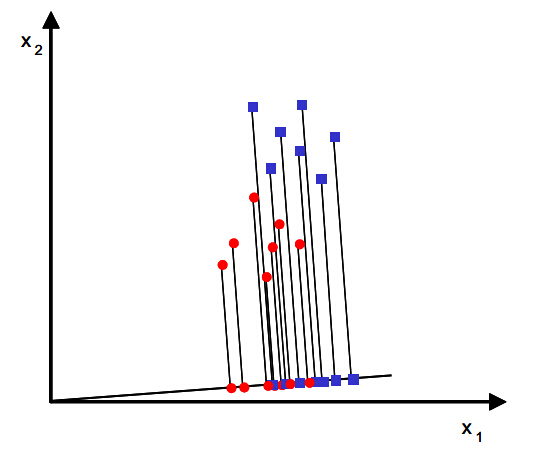
\includegraphics[width=0.3\textwidth]{LDAsimple_a.jpg}}
\hspace{0.2in}
\subfigure[]{
\label{fig:b}
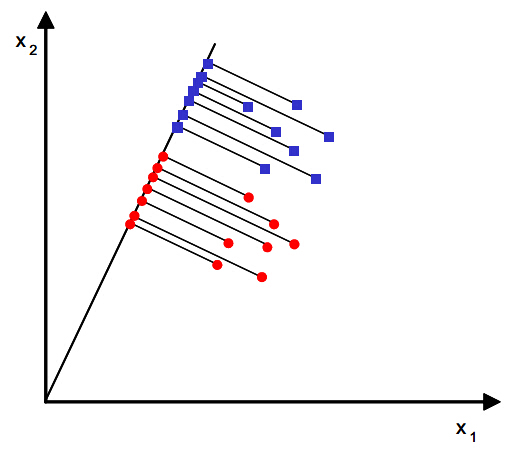
\includegraphics[width=0.3\textwidth]{LDAsimple_b.jpg}}
\caption{LDA����ά�ռ����������(�ֱ���Ϊ�졢����ɫ)��Ͷ�䵽һάʾ��ͼ����ͼ\ref{fig:a}������Ͷ�䵽һά�ռ�������������ݵ㽻����һ�𣬸�����ж��������ѣ�����ͼ\ref{fig:b}Ͷ�䵽һά�ռ����������ж���Ϣ���ܹ���һά�ռ�ܺõؽ��з��࣬LDA�����ҵ���ѵ�Ͷ�䷽��}
\label{fig:LDAsample}
\end{figure}
\subsection{��������}
���ȶ������ݼ�����������$\bm{x}\in \mathcal{R}^n$������ǩ$\{c_1,c_2\}$��Ҫ��IJ�������Ͷ�亯��ʽ\ref{equ:project}�е�Ͷ������$\bm{w}\in \mathcal{R}^n$����Ϊ�Ƕ��������⣬����Ͷ������$\bm{w}$ֻ��һ���������$c_1$��ʵ����Ŀ$n_1$��$c_2$��ʵ����Ŀ$n_2$��$N=n_1+n_2$���ٶ������
\begin{eqnarray}
  \bm{\mu_1}=&\frac{1}{n_1}\sum_{\bm{x}\in c_1}{\bm{x}}\\
  \bm{\mu_2}=&\frac{1}{n_2}\sum_{\bm{x}\in c_2}{\bm{x}}\\
  \bm{\mu}=&\frac{1}{N}\sum_{\forall \bm{x}}{\bm{x}}=\frac{1}{N}\left(n_1\bm{\mu_1}+n_2\bm{\mu_2}\right)
\end{eqnarray}
����$\mu_1,\mu_2$�ֱ������$c_1,c_2$��ʵ�����������������ĵ㣬$\mu$������ʵ�������ĵ㡣
��Ͷ�䵽һά����������ĵ�
\begin{eqnarray}
  \widetilde{\mu_1}&=\bm{w}^T\mu_1=\frac{1}{n_1}\sum_{\bm{x}\in c_1}{\bm{w}^T\bm{x}}\\
  \widetilde{\mu_2}&=\bm{w}^T\mu_2=\frac{1}{n_2}\sum_{\bm{x}\in c_2}{\bm{w}^T\bm{x}}\\
  \widetilde{\mu}&=\frac{1}{N}\sum_{\forall \bm{x}}{\bm{w}^T\bm{x}}=\frac{1}{N}\left(n_1\widetilde{\mu_1}+n_2\widetilde{\mu_2}\right)
\end{eqnarray}

���Ƕ����ʼ������������ڵ�ʵ�������������ķ�ɢ�̶ȵĶ���$S_1,S_2$
\begin{eqnarray}
  S_1&=\sum_{\bm{x}\in c_1}(\bm{x}-\bm{\mu}_1)(\bm{x}-\bm{\mu}_1)^T\\
  S_2&=\sum_{\bm{x}\in c_2}(\bm{x}-\bm{\mu}_1)(\bm{x}-\bm{\mu}_1)^T
\end{eqnarray}
�ڴ˻����϶����ʼ�����ܵ�����ڵ�ʵ�������������ķ�ɢ�̶ȵĶ���$S_W$
\begin{equation}\label{equ:SW}
  S_W=S_1+S_2=\sum_{i=1}^{2}\sum_{\bm{x}\in c_i}(\bm{x}-\bm{\mu}_i)(\bm{x}-\bm{\mu}_i)^T
\end{equation}
Ȼ�����Ƕ����ʼ��������ķ�ɢ�̶ȵĶ���$S_B$
\begin{equation}\label{equ:SB}
  S_B=(\bm{\mu}_1-\bm{\mu}_2)(\bm{\mu}_1-\bm{\mu}_2)^T
\end{equation}

ͶӰ�������ڵķ�ɢ�̶ȵĶ���$\widetilde{S_W}$
\begin{equation}
\begin{split}
  \widetilde{S_W}   &=\sum_{i=1}^{2}\sum_{c\in c_i}(y-\mu_i)(y-\mu_i)^T\\
                    &=\sum_{i=1}^{2}\sum_{c\in c_i}(\bm{w}^T\bm{x}-\bm{w}^T\bm{\mu}_i)(\bm{w}^T\bm{x}-\bm{w}^T\bm{\mu}_i)^T\\
                    &=\sum_{i=1}^{2}\sum_{c\in c_i}\bm{w}^T(\bm{x}-\bm{\mu}_i)(\bm{x}-\bm{\mu}_i)^T\bm{w}\\
                    &=\bm{w}^T\left(\sum_{i=1}^{2}\sum_{c\in c_i}(\bm{x}-\bm{\mu}_i)(\bm{x}-\bm{\mu}_i)^T\right)\bm{w}\\
                    &=\bm{w}^TS_W\bm{w}
\end{split}
\end{equation}
ͶӰ�������ķ�ɢ�̶ȵĶ���$\widetilde{S_B}$
\begin{equation}
\begin{split}
  \widetilde{S_B}   &=(\widetilde{\mu_1}-\widetilde{\mu_2})(\widetilde{\mu_1}-\widetilde{\mu_2})^T \\
        &=(\bm{w}^T\bm{\mu}_1-\bm{w}^T\bm{\mu}_2)(\bm{w}^T\bm{\mu}_1-\bm{w}^T\bm{\mu}_2)^T\\
        &=\bm{w}^T S_B\bm{w}
\end{split}
\end{equation}

����ͶӰ���ʵ��������ɢ�̶�(��$\widetilde{S_B}$)Խ�����ڷ�ɢ�̶�(��$\widetilde{S_W}$)ԽС��Ч��Խ�ã��������Ƕ�������ģ�����ۺ���
\begin{equation}\label{equ:LDA2J}
\begin{split}
  J(\bm{w})=\frac{\widetilde{S_B}}{\widetilde{S_W}}=\frac{\bm{w}^T S_B\bm{w}}{\bm{w}^T S_W\bm{w}}
\end{split}
\end{equation}

ʽ\ref{equ:LDA2J}�ǹ���ͶӰ����$\bm{w}$�ĺ��������Ӻͷ�ĸ���DZ��������Ҿ���$S_B,S_W$�������ù�ʽ\ref{equ:SB},\ref{equ:SW} ���ݳ�ʼ����ֱ�Ӽ���ó��������������ʽ\ref{equ:LDA2J}�õ���ѵ�ͶӰ����$\bm{w}$��Ŀ�꺯����
\begin{equation}\label{equ:LDAarg}
\bm{w}^{*}=\arg\min_{\bm{w}}-\frac{\bm{w}^T S_B\bm{w}}{\bm{w}^T S_W\bm{w}}
\end{equation}

�۲�ʽ\ref{equ:LDA2J}������һ������$\bm{w}$�ij߶ȸı���ı�������������ǿ��ԼӸ��������޶�$\bm{w}$�ij߶ȣ���򵥵ģ��涨$\bm{w}^T S_W\bm{w}=1$����Ŀ�꺯����дΪ
\begin{equation}\label{equ:LDAarg2}
\begin{split}
\bm{w}^{*}&=\arg\min_{\bm{w}}-\frac{1}{2}\bm{w}^T S_B\bm{w}\\
            & s.t.\quad\bm{w}^T S_W\bm{w}=1
\end{split}
\end{equation}
����֮���ԼӸ�ϵ��$\frac{1}{2}$ֻ��Ϊ�˷����ߵ��󵼡�

ʽ\ref{equ:LDAarg2}��Ӧ��Lagrangian��ʽ
\begin{equation}
  \mathcal{L}_J=-\frac{1}{2}\bm{w}^T S_B\bm{w}+\frac{1}{2}\lambda \left(\bm{w}^T S_W\bm{w}-1\right)
\end{equation}

KKT����������������Ľ�$\bm{w}^{*}$������
\begin{equation}
  \frac{\partial \mathcal{L}_J}{\partial \bm{w}^{*}}=S_B\bm{w}^{*}-\lambda S_W\bm{w}^{*}=0\Rightarrow S_B\bm{w}^{*}=\lambda S_W\bm{w}^{*}
\end{equation}

���ھ���$S_B$��ʵ�Գƾ��󣬸��ݵ�\ref{subsec:symetric}�ڣ������ǿ���ģ�������
\begin{equation}
  S_W^{-1}S_B\bm{w}^{*}=\lambda \bm{w}^{*}
\end{equation}
���������������$n$�׾���$S_W^{-1}S_B$������������

���ھ���$S_B��S_W$����ʵ�Գƾ�������$S_W^{-1}S_B$Ҳ��ʵ�Գƾ��󣬸��ݵ�\ref{subsec:symetric}�ڣ�����$n$����������������������ȡ$S_W^{-1}S_B$����������ֵ$\lambda^{*}$ ����Ӧ������������Ϊ��ѵ�ͶӰ����$\bm{w}^{*}$��

�������֤���������о���$S_W^{-1}S_B$������ֵ$\lambda$�����Ӧ����������$\bm{w}$��������뵽ʽ\ref{equ:LDA2J}���õ�
\begin{equation}
  \begin{split}
    J(\bm{w})&=\frac{\bm{w}^T S_B\bm{w}}{\bm{w}^T S_W\bm{w}}\\
            &=\bm{w}^T S_B\bm{w}\\
            &=\lambda\bm{w}S_W\bm{w}\\
            &=\lambda
  \end{split}
\end{equation}
Ҳ����˵��$J(\bm{w})$�Ĵ�С��������ֵ$\lambda$�������ܹ����$J(\bm{w})$��$\bm{w}^{*}$Ϊ$S_W^{-1}S_B$����������ֵ$\lambda^{*}$����Ӧ������������
\subsection{��������}
��LDA��չ�����ڶ���ࣨ��$c$��������⣬������������һС�ڵ�ͶӰ������$\bm{w}$��˼·����һС�ڵĶ����������ͬ���������漸�������Ķ��巽����û�иı�
\begin{eqnarray}
  \bm{\mu}_i&=\frac{1}{n_i}\sum_{\bm{x}\in c_i}{\bm{x}}\\
  \bm{\mu}&=\frac{1}{N}\sum_{\forall \bm{x}}{\bm{x}}=\frac{1}{N}\sum_{i=1}^{c}n_i\bm{\mu}_i\\
  \widetilde{\bm{\mu}_i}&=\frac{1}{n_i}\sum_{\bm{x}\in c_i}{\bm{w}^T\bm{x}}\\
  \widetilde{\bm{\mu}}&=\frac{1}{N}\sum_{\forall \bm{x}}{\bm{w}^T\bm{x}}=\frac{1}{N}\sum_{i=1}^{c}n_i\bm{w}^T\bm{\mu}_i\\
  S_i&=\sum_{\bm{x}\in c_i}(\bm{x}-\bm{\mu}_i)(\bm{x}-\bm{\mu}_i)^T\\
  S_W&=\sum_{i=1}^{c}S_i=\sum_{i=1}^{c}\sum_{\bm{x}\in c_i}(\bm{x}-\bm{\mu}_i)(\bm{x}-\bm{\mu}_i)^T\\
  \widetilde{S_W}&=\bm{w}^TS_W\bm{w}\\
  \widetilde{S_B}&=\bm{w}^TS_B\bm{w}
\end{eqnarray}
ֻ�о���$S_B$�Ķ��������޸ģ����¶�������
\begin{equation}
  S_B=\sum_{i=1}^{c}n_i(\bm{\mu}_i-\bm{\mu})(\bm{\mu}_i-\bm{\mu})^T
\end{equation}
����һ����ͬ�ڶ�����������ǣ�$c$�����������ѡȡ���$c-1$����������(��Ȼ������$c-1$������ֵ����Ӧ����������)��������������ѡȡ$k(k\leq c-1)$��������������$k$ �����������þ����ʾΪ
\begin{equation}
  \bm{w}=(\bm{w}_1,\bm{w}_2,\cdots,\bm{w}_k)
\end{equation}
��ʵ��$\bm{x}$�Ϳ���������ķ�ʽӳ�䵽һ��$k$ά������
\begin{equation}
  \bm{y}=\bm{w}^T\bm{x}
\end{equation}
Ȼ�����ǾͿ���ͨ���Ե�ά�ռ䣨$k$������������$\bm{y}$�ķ������ﵽ�Ը�ά�ռ䣨$n$����������$x$���з����Ŀ�ġ�
\subsection{LDA�ľ���}
LDA���������������ڲ���ʵ����ѭ��˹�ֲ���unimodal Gaussian����������ǣ�Ҳ����˵��������б��������йصĸ��ӵĽṹ��Ϣ��LDA ���������ڽ�ά�Ĺ����а���Щ�����Ϣ�������Ӷ��ò���ʧ��ͼ\ref{fig:LDAcase}�ļ������������LDA����
\begin{figure}[!ht]
\centering
\subfigure[]{
\label{fig:c1}
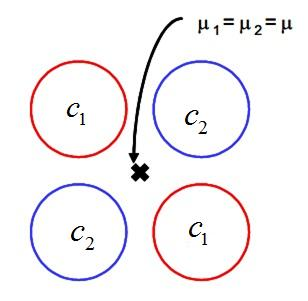
\includegraphics[width=0.3\textwidth]{LDAcase1.jpg}}
\hspace{0.1in}
\subfigure[]{
\label{fig:c2}
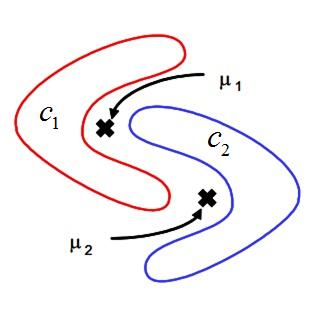
\includegraphics[width=0.3\textwidth]{LDAcase2.jpg}}
\hspace{0.1in}
\subfigure[]{
\label{fig:c3}
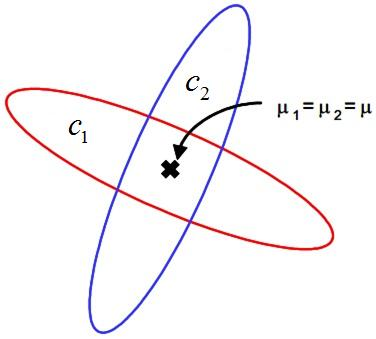
\includegraphics[width=0.3\textwidth]{LDAcase3.jpg}}
\caption{��ͼ\ref{fig:c1}���������(�ֱ��ú졢��������ɫ����)�ֱ���������ֵ��ͬ��˹�ֲ���ɣ�����unimodal Gaussian ���Բ�����LDA;��ͼ\ref{fig:c2}�ķֲ�Ҳ���Ǹ�˹�ֲ�;��ͼ��ͼ\ref{fig:c3}�������ֲ��ľ�ֵ��ȣ��⽫ʹʽ\ref{equ:LDA2J}��Ϊ0������Ҳ������LDA}
\label{fig:LDAcase}
\end{figure}
\section{PCA}\label{sec:PCA}
PCA�������ɷַ�����Principal components analysis������һ��unsupervised learning����Ҫ��������Ԥ�����е�������ȡ���ڣ������ݼ���Ϊ�����ٵ���Ч��������ʾ��ͬʱʹ��ԭ����������Ϣ�����ܵı�����
\subsection{PCA�㷨}
���õ�\ref{subsec:cov}С�ڣ�Э������󣩵����ӣ����Ǵ�ij��ʵ���еõ���ͬ���͵�$N$����¼����$\bm{x}_1,\bm{x}_2,\cdots,\bm{x}_N$��ÿ����¼����$M$ ά������������Ӧ��$M$ �������������������ǽ���һ����PCA����ȡ������Ч��������ά�Ĺ��̡�
\begin{enumerate}
  \item ��$M\times N$�׵ľ���$\bm{A}=\left(\bm{x}_1,\bm{x}_2,\cdots,\bm{x}_N\right)$�������ݣ�����$\bm{A}$��Э������󣨷�������\ref{subsec:cov}�����õ�$M\times M$��Э�������$\bm{\Sigma}$
  \item ��$\bm{\Sigma}$��������ֵ�ֽ⣨��������\ref{subsec:deco}��������$\bm{\Sigma}$��Э������󣬸��ݵ�\ref{subsec:symetric}С�ڵĽ��ۣ��صõ�$M$��������(�����ظ�)������С��������$\lambda_1\geq\lambda_2\geq\cdots\geq\lambda_M$���Լ���Ӧ����������$\bm{\nu}_1,\bm{\nu}_2,\cdots,\bm{\nu}_M$��
  \item ��ǰ���ѡ��$k$����Ҳ��������$k$������ֵ$\lambda_1\geq\lambda_2\geq\cdots\geq\lambda_k$��Ӧ���������������$M\times k$�׵ľ���$\bm{w}=(\bm{\nu}_1,\bm{\nu}_2,\cdots,\bm{\nu}_k)$��
  \item ����$\bm{w}^T\times\bm{A}$���õ�$k\times N$�ľ��󣬽�����Ϊ$\widetilde{\bm{A}}$����$\widetilde{\bm{A}}$����PCA ��ά������ݾ���
\end{enumerate}

ѡȡ��ǰ$k$�����ɷ֣����������������ۼƹ����ʵļ��㷽��
\begin{equation}
  \eta =\frac{\sum_{i=1}^{k}\lambda_i}{\sum_{i=1}^{M}\lambda_i}
\end{equation}
��������ʾ��������Ϣ�ı��أ���������$k$�����ɷ�������ԭʼ���ݵ����������ԭʼ��ά��֮����нϸߵ�����ԣ���ǰ�������������ɷֵ��ۻ�������ͨ�����ܴﵽһ���ϸߵ�ˮƽ��

\subsection{��󻯷������PCA}
���źŴ�������Ϊ�źž��нϴ�ķ�������н�С�ķ������Ⱦ����ź��������ķ���֮�ȣ�Խ��Խ�á����Բο�ͼ\ref{fig:PCAvar} ����������ø��
\begin{figure}[!ht]
  \centering
  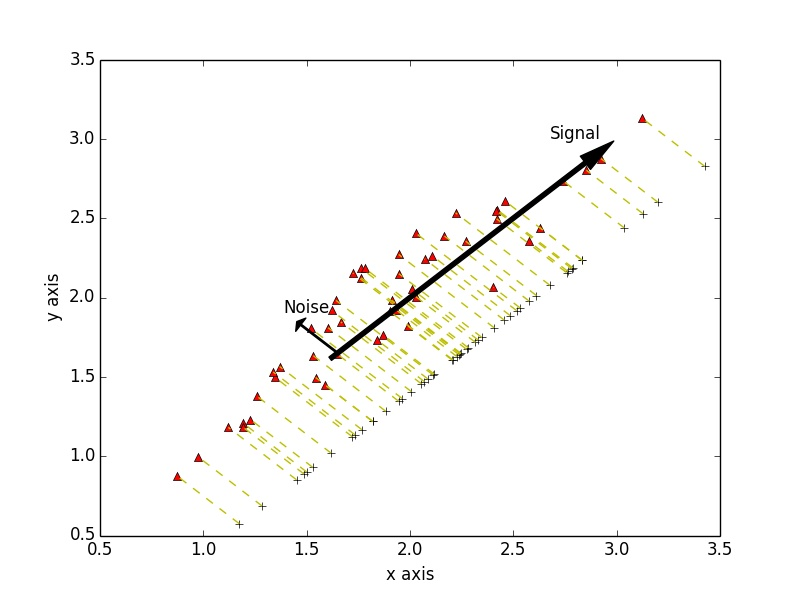
\includegraphics[width=0.6\textwidth,height=0.5\textwidth]{PCA_sample.jpg}
  \caption{��󻯷���ʾ��ͼ��ͼ�еĺ�ɫ�����Ǽ�CE�����źţ����Կ����������ضԽ��߷ֲ�����ͼʾ�Ľϴֵļ�ͷָʾ�ķ��򣩣���CE�ź��ظ÷����ͶӰ��ͼʾ�IJ����γɵ��ߣ����Կ�������ʵ���źţ�Signal���������Եĸ�ͶӰ���ݷ�����󡣶���ֱ�ڸ÷����ͶӰ����ͼʾ�Ľ�ϸ�ļ�ͷָʾ�ķ���ͶӰ����δ���������Կ���������(Noise)�����ǿ��������������ݣ�ֻ��ȡ�ڷ���������ϵ�ͶӰ���ݣ���ʵ������һά���ݱ�ʾԭ���Ķ�ά���ݣ��������PCA����ά�Ļ���ԭ����}
  \label{fig:PCAvar}
\end{figure}

���ɷ���������Ͷ������$\bm{w}$������ͶӰ��$\bm{w}$��֮�󱻹㷺ɢ����ʹ������֮��IJ���������ԣ�����󻯷��

���һ��Ͷ������$\bm{w}_1$������ǰ��Ľ�����ԭʼ����Ͷ�䵽�÷���õ���������Ϊ
\begin{equation*}
  \widetilde{\bm{x}}=\left(\bm{w}_1^T\bm{x}_1,\bm{w}_1^T\bm{x}_2,\bm{w}_1^T\bm{x}_3,\cdots,\bm{w}_1^T\bm{x}_N,\right)
\end{equation*}
$\widetilde{\bm{x}}$������
\begin{equation}
  \widetilde{\mu}=\frac{1}{N}\sum_{i=1}^{N}\bm{w}_1^T\bm{x}_i
\end{equation}
��$\widetilde{\bm{x}}$�ķ���
\begin{equation}
\begin{split}
  \widetilde{\bm{\Sigma}}&=\frac{1}{N}\sum_{i=1}^{N}(\bm{w}_1^T\bm{x}_i-\widetilde{\mu})^T(\bm{w}_1^T\bm{x}_i-\widetilde{\mu})\\
                         &=\bm{w}_1^T\left(\frac{1}{N}\sum_{i=1}^{N}(\bm{x}_i-\widetilde{\mu})^T(\bm{x}_i-\widetilde{\mu})\right)\bm{w}_1\\                    &=\bm{w}_1^T\bm{\Sigma}\bm{w}_1
\end{split}
\end{equation}
����$\bm{\Sigma}$����ԭʼ���ݵķ������
�����ǵ�����ת����
\begin{equation}
  \begin{split}
    \bm{w}_1^{*}=&\quad\arg\max_{\bm{w}_1} \quad\bm{w}_1^T\bm{\Sigma}\bm{w}_1\\
                    &\bm{w}_1^T\bm{w}_1=1
  \end{split}
\end{equation}
���Ӧ��Lagrangian��ʽ
\begin{equation}\label{equ:PCA_larg}
  \mathcal{L}_J\left(\bm{w}_1\right)=-\frac{1}{2}\bm{w}_1^T\bm{\Sigma}\bm{w}_1+\frac{1}{2}\lambda \left(\bm{w}_1^T\bm{w}_1-1\right)
\end{equation}
��$\mathcal{L}_J$����$\bm{w}_1$��Ϊ0����
\begin{equation}
  \frac{\partial\mathcal{L}_J\left(\bm{w}_1\right)}{\partial\bm{w}_1 }=-\bm{\Sigma}\bm{w}_1+\lambda\bm{w}_1 = 0 \Rightarrow \bm{\Sigma}\bm{w}_1=\lambda\bm{w}_1
\end{equation}
��$\bm{\Sigma}\bm{w}_1=\lambda\bm{w}_1$��$\bm{w}_1^T\bm{w}_1=1$����ʽ\ref{equ:PCA_larg}��
\begin{equation}
  \mathcal{L}_J\left(\bm{w}_1\right)=-\frac{1}{2}\bm{w}_1^T\bm{\Sigma}\bm{w}_1=-\frac{1}{2}\bm{w}_1^T\lambda_1\bm{w}_1=-\frac{1}{2}\lambda_1
\end{equation}
���Կ�������һ�����ɷ�$\bm{w}_1^{*}$Ӧ��ȡΪ�������$\bm{\Sigma}$�������ֵ����Ӧ��������������������ֵ$\lambda_1^{*}$ ���Ǹ����ɷ���ԭʼ���ݵĹ����ʡ�

����õ�һ�����ɷ�$\bm{w}_1^{*}$�Ļ����ϣ����������һ�����ɷ�$\bm{w}_2$��$\bm{w}_2$����$\bm{w}_1^{*}$������ʹ��Ͷ�������ϵ����ݵķ�������Ͷ��������Ϊ�˼򻯷��ţ����ǰѵ�һ�����ɷ�$\bm{w}_1^{*}$���Ϊ$\bm{w}_1$�����Ӧ������ֵ$\lambda_1^{*}$���Ϊ���Ϊ$\lambda_1$���ο�������Ƶ��õ��Ż�Ŀ��
\begin{equation}
  \begin{split}
    \bm{w}_2^{*}=&\quad\arg\max_{\bm{w}_2} \quad\bm{w}_2^T\bm{\Sigma}\bm{w}_2\\
                    &\bm{w}_2^T\bm{w}_2=1\\
                    &\bm{w}_2^T\bm{w}_1=0
  \end{split}
\end{equation}
��Ӧ��Lagrangian��ʽ
\begin{equation}\label{equ:PCA_larg2}
  \mathcal{L}_J\left(\bm{w}_2\right)=-\frac{1}{2}\bm{w}_2^T\bm{\Sigma}\bm{w}_2+\frac{1}{2}\lambda \left(\bm{w}_2^T\bm{w}_2-1\right)+\beta\left(\bm{w}_2^T\bm{w}_1-0\right)
\end{equation}
��$\mathcal{L}_J\left(\bm{w}_2\right)$����$\bm{w}_2$��Ϊ0����
\begin{equation}\label{equ:PCA_beta}
  \bm{\Sigma}\bm{w}_2-\lambda\bm{w}_2-\beta\bm{w}_1=0
\end{equation}
����ʽ���$\bm{w}_1^T$����
\begin{equation}
  \bm{w}_1^T\bm{\Sigma}\bm{w}_2-\lambda\bm{w}_1^T\bm{w}_2-\beta\bm{w}_1^T\bm{w}_1=0
\end{equation}
ȥ��Ϊ$0$������
\begin{equation}\label{equ:PCA_beta0}
  \bm{w}_1^T\bm{\Sigma}\bm{w}_2-\beta\bm{w}_1^T\bm{w}_1=0
\end{equation}
����$\bm{w}_1^T\bm{\Sigma}\bm{w}_2$Ϊ������Э�������$\bm{\Sigma}$Ϊ�Գƾ���������
\begin{equation}
  \bm{w}_1^T\bm{\Sigma}\bm{w}_2=\left(\bm{w}_1^T\bm{\Sigma}\bm{w}_2\right)^T=\bm{w}_2^T\bm{\Sigma}\bm{w}_1=\bm{w}_2^T\lambda_1\bm{w}_1=0
\end{equation}
��$\bm{w}_1^T\bm{\Sigma}\bm{w}_2=0$����ʽ\ref{equ:PCA_beta0}֪$\beta=0$����$\beta=0$����ʽ\ref{equ:PCA_beta}���õ�ʽ
\begin{equation}\label{equ:PCA_eign2}
  \bm{\Sigma}\bm{w}_2=\lambda\bm{w}_2
\end{equation}
��ʽ\ref{equ:PCA_eign2}֪$\bm{w}_2$��$\bm{\Sigma}$��һ������������$\lambda$��$\bm{w}_2$��Ӧ������ֵ��
��ʽ\ref{equ:PCA_eign2}����ʽ\label{equ:PCA_larg2}�������ǰ��������ͽ��ۣ��õ�
\begin{equation}
  \mathcal{L}_J\left(\bm{w}_2\right)==-\frac{1}{2}\lambda_2
\end{equation}
������ڶ������ɷ�$\bm{w}_2^{*}$Ӧ���Ǵδ������ֵ$\lambda_2^{*}$��Ӧ������������

����ǰ������󻯷������õ�һ���ڶ����ɷֵķ��������ǿ���������ú��������ɷ֡�PCA��ȫ�������򵥵�˵�����Ƕ�ԭʼ�Ŀռ���˳�����һ���໥�����������ᣬ��һ������ʹ�÷������ģ��ڶ������������һ����������ƽ����ʹ�÷������ģ����������������1$,2$ ����������ƽ���з������ģ�����������$N$ά�ռ��У����ǿ����ҵ�$N$�������������ᣬ����ȡǰ$k$��ȥ��������ռ䣬�����ʹ�һ��$N$ ά�Ŀռ�ѹ����$k$ά�Ŀռ��ˣ���������ѡ���$k$���������ܹ�ʹ�ÿռ��ѹ��ʹ�����ݵ���ʧ��С��
\subsection{��С����ʧ����PCA}
��С����ʧ����һ���ǶȽ���PCAΪʲôҪ����������ֵ����Ӧ���������������ǣ�Ϊ����С����ʧ��

�����Ѿ��ҵ���$N$����λ��������$\bm{w}_1,\bm{w}_2,\cdots,\bm{w}_N$����ʾ$N$ά������$\bm{x}$������
\begin{equation}
  \bm{x_n}=\sum_{i=1}^{N}\left(\bm{x_n}^T\bm{w}_i\right)\bm{w}_i
\end{equation}
�����ǵ��������$\widetilde{\bm{x}}_n$������ԭ���ĵ�$\bm{x}_n$
\begin{equation}\label{equ:PCA_near}
  \widetilde{\bm{x}}_n=\sum_{i=1}^{K}z_{ni}\bm{w}_i+\sum_{i=K+1}^{N}b_i\bm{w}_i
\end{equation}
�۲�ʽ\ref{equ:PCA_near}��ע��$z_{ni}$��ÿ��$x_n$���Dz�ͬ�ģ���$b_i$�����е�$x_n$������ͬ�ġ����������һ�㣬�㽫�����ڶԺ�����󵼲�֪���롣���⣬����$b_i$�����е�$x_n$�����޲��ģ�����˵$b_i$��������$x_n$�޹صģ���PCA������ά�����ǽ���������Щ��Ϣ����$z_{ni}$��$x_n$֮��IJ��컯��Ϣ��������ά��õ��ľ���$z_{ni}$��ʽ\ref{equ:PCA_near}��ʾ��PCA�����ݴ�ԭ����$N$ ά�ռ併��$K$ά�ռ䡣

PCA��ά�϶���ʧ��һЩ��Ϣ��������ʧ������ʽ��Ϊ
\begin{equation}
\begin{split}
  J(z,b)&=\frac{1}{N}\sum_{n=1}^{N}||\bm{x}_n-\widetilde{\bm{x}_n}||^2\\
        &=\frac{1}{N}\sum_{n=1}^{N}||\sum_{i=1}^{K}z_{ni}\bm{w}_i+\sum_{i=K+1}^{N}b_i\bm{w}_i-\bm{x}_n||^2\\
        &=\frac{1}{N}\sum_{n=1}^{N}\left(\sum_{i=1}^{K}z_{ni}\bm{w}_i+\sum_{i=K+1}^{N}b_i\bm{w}_i-\bm{x}_n\right)^T\left(\sum_{i=1}^{K}z_{ni}\bm{w}_i+\sum_{i=K+1}^{N}b_i\bm{w}_i-\bm{x}_n\right)
\end{split}
\end{equation}
Ҫ����ʧ����$J(z,b)$��С��������ж�$z,b$��Ϊ$0$���������󵼹��̡�
\begin{equation}
\begin{split}
  \frac{\partial J(z,b)}{\partial z_{nj}}&=\frac{1}{N}\left(\sum_{i=1}^{K}z_{ni}\bm{w}_i+\sum_{i=K+1}^{N}b_i\bm{w}_i-\bm{x}_n\right)^T\bm{w}_j\\
        &=\frac{1}{N}\left(\sum_{i=1}^{K}z_{ni}\bm{w}_i^T\bm{w}_j+\sum_{i=K+1}^{N}b_i\bm{w}_i^T\bm{w}_j-\bm{x}_n^T\bm{w}_j\right)\\
        &=\frac{1}{N}\left(z_{nj}\bm{w}_j^T\bm{w}_j-\bm{x}_n^T\bm{w}_j\right)\\
        &=\frac{1}{N}\left(z_{nj}-\bm{x}_n^T\bm{w}_j\right)=0
\end{split}
\end{equation}
�õ�
\begin{equation}\label{equ:PCA_znj}
  z_{nj}=\bm{x}_n^T\bm{w}_j
\end{equation}
\begin{equation}
\begin{split}
  \frac{\partial J(z,b)}{\partial b_{j}}&=\frac{1}{N}\sum_{n=1}^{N}\left(\sum_{i=1}^{K}z_{ni}\bm{w}_i+\sum_{i=K+1}^{N}b_i\bm{w}_i-\bm{x}_n\right)^T\bm{w}_j\\
        &=\frac{1}{N}\sum_{n=1}^{N}\left(b_j\bm{w}_j^T\bm{w}_j-\bm{x}_n^T\bm{w}_j\right)\\
        &=\frac{1}{N}\sum_{n=1}^{N}\left(b_j-\bm{x}_n^T\bm{w}_j\right)\\
        &=b_j-\frac{1}{N}\sum_{n=1}^{N}\bm{x}_n^T\bm{w}_j\\
        &=b_j-\left(\frac{1}{N}\sum_{n=1}^{N}\bm{x}_n^T\right)\bm{w}_j\\
        &=b_j-\left(\frac{1}{N}\sum_{n=1}^{N}\bm{x}_n\right)^T\bm{w}_j\\
        &=b_j-\bm{\mu}^T\bm{w}_j=0
\end{split}
\end{equation}
�õ�
\begin{equation}\label{equ:PCA_bj}
  b_j=\bm{\mu}^T\bm{w}_j
\end{equation}

��ʽ\ref{equ:PCA_znj}��ʽ\ref{equ:PCA_bj}������$\bm{x}_n-\widetilde{\bm{x}_n}$
\begin{equation}
  \begin{split}
    \widetilde{\bm{x}_n}-\bm{x}_n&=\sum_{i=1}^{K}z_{ni}\bm{w}_i+\sum_{i=K+1}^{N}b_i\bm{w}_i-\bm{x}_n\\
                &=\sum_{i=1}^{K}\left(\bm{x}_n^T\bm{w}_i\right)\bm{w}_i+\sum_{i=K+1}^{N}\left(\bm{\mu}^T\bm{w}_i\right)\bm{w}_i-\bm{x}_n\\
                &=\sum_{i=1}^{K}\left(\bm{x}_n^T\bm{w}_i\right)\bm{w}_i+\sum_{i=K+1}^{N}\left(\bm{\mu}^T\bm{w}_i\right)\bm{w}_i-\sum_{i=1}^{N}\left(\bm{x}_n^T\bm{w}_i\right)\bm{w}_i\\
                &=\sum_{i=K+1}^{N}\left(\bm{\mu}^T\bm{w}_i\right)\bm{w}_i-\sum_{i=K+1}^{N}\left(\bm{x}_n^T\bm{w}_i\right)\bm{w}_i\\
                &=\sum_{i=K+1}^{N}\left(\left(\bm{\mu}-\bm{x}_n\right)^T\bm{w}_i\right)\bm{w}_i
  \end{split}
\end{equation}

������ʧ��������
\begin{equation}
  \begin{split}
      J(z,b)&=\frac{1}{N}\sum_{n=1}^{N}\left(\sum_{i=K+1}^{N}\left(\left(\bm{\mu}-\bm{x}_n\right)^T\bm{w}_i\right)\bm{w}_i\right)^T\left(\sum_{i=K+1}^{N}\left(\left(\bm{\mu}-\bm{x}_n\right)^T\bm{w}_i\right)\bm{w}_i\right)\\
      &=\frac{1}{N}\sum_{n=1}^{N}\sum_{i=K+1}^{N}\left(\left(\bm{\mu}-\bm{x}_n\right)^T\bm{w}_i\right)^2\bm{w}_i^T\bm{w}_i\\
      &=\frac{1}{N}\sum_{n=1}^{N}\sum_{i=K+1}^{N}\left(\left(\bm{\mu}-\bm{x}_n\right)^T\bm{w}_i\right)^2\\
      &=\sum_{i=K+1}^{N}\frac{1}{N}\sum_{n=1}^{N}\left(\left(\bm{\mu}-\bm{x}_n\right)^T\bm{w}_i\right)^2\\
      &=\sum_{i=K+1}^{N}\frac{1}{N}\sum_{n=1}^{N}\left(\left(\bm{\mu}-\bm{x}_n\right)^T\bm{w}_i\right)^T\left(\left(\bm{\mu}-\bm{x}_n\right)^T\bm{w}_i\right)\\
      &=\sum_{i=K+1}^{N}\frac{1}{N}\sum_{n=1}^{N}\bm{w}_i^T\left(\bm{\mu}-\bm{x}_n\right)\left(\bm{\mu}-\bm{x}_n\right)^T\bm{w}_i\\
      &=\sum_{i=K+1}^{N}\bm{w}_i^T\left(\frac{1}{N}\sum_{n=1}^{N}\left(\bm{\mu}-\bm{x}_n\right)\left(\bm{\mu}-\bm{x}_n\right)^T\right)\bm{w}_i\\
      &=\sum_{i=K+1}^{N}\bm{w}_i^T\bm{\Sigma}\bm{w}_i\\
      &=\sum_{i=K+1}^{N}\bm{w}_i^T\lambda_i\bm{w}_i\\
      &=\sum_{i=K+1}^{N}\lambda_i
  \end{split}
\end{equation}
����Ҫʹ��ʧ����$J$��С��ֻҪ��δѡȡ��N-K��������������Ӧ������ֵ�ĺ���С����������Ҫѡȡ����$K$������ֵ��Ӧ������������Ϊ���ɷֲ���ʹPCA��ʧ��С��




\section{SVD}
SVD(Singular Value Decomposition)�����������������ֵ�ֽ⣬�����Խ�һ���Ƿ����һ�����ֽ����������ij˵���ʽ���������ھ���������ȡ����ά��ѹ���ȵȡ�
\subsection{���������SVD}
����һ�������������ȴӶ��׷�����˵�𣬽��þ�����$\bm{A}$��ʾ���ش��������ĵ�λ������$\bm{v}_1,\bm{v}_2$(��ͼ\ref{fig:SVD})������$\bm{A}\bm{v}_1$ ��$\bm{A}\bm{v}_2$Ҳ�������ġ�
\begin{figure}[!ht]
\centering
\subfigure[]{
\label{fig:SVDa}
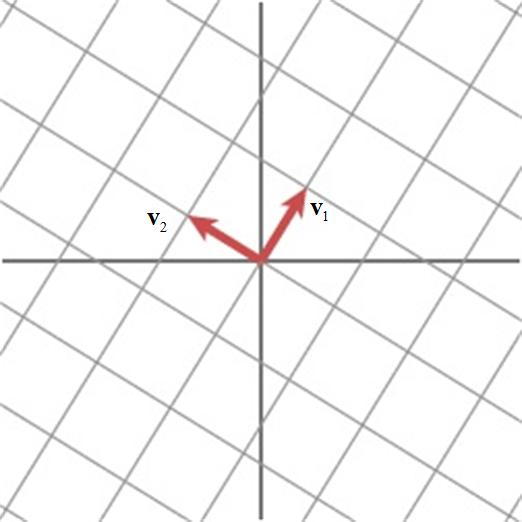
\includegraphics[width=0.3\textwidth]{SVD_intro1.jpg}}
\hspace{0.2in}
\subfigure[]{
\label{fig:SVDb}
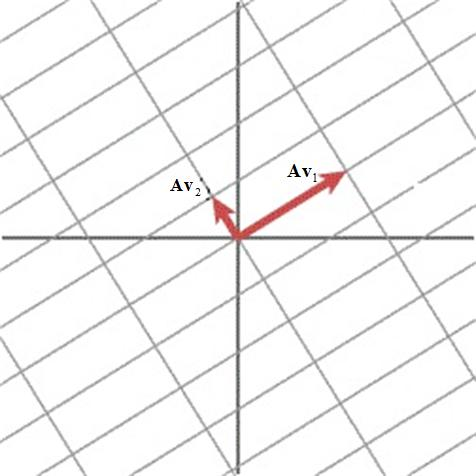
\includegraphics[width=0.3\textwidth]{SVD_intro2.jpg}}
\caption{����һ���׷�����$\bm{A}$���ش��������ĵ�λ������$\bm{v}_1,\bm{v}_2$������$\bm{A}\bm{v}_1$ ��$\bm{A}\bm{v}_2$Ҳ�������ġ�}
\label{fig:SVD}
\end{figure}
��$\bm{A}\bm{v}_1=\sigma_1\bm{u}_1,\bm{A}\bm{v}_2=\sigma_2\bm{u}_2$������$\bm{u}_1,\bm{u}_2$Ϊ��λ��������ʽ���������£�
\begin{equation}
  \begin{split}
    \forall \bm{A},\exists \bm{A}\bm{v}_1=\sigma_1\bm{u}_1,&\bm{A}\bm{v}_2=\sigma_2\bm{u}_2\\
                    s.t.\quad   &\bm{v}_1^T\bm{v}_2=0,\bm{u}_1^T\bm{u}_2=0\\
                                &||\bm{v}_1||=||\bm{v}_2||=||\bm{u}_1||=||\bm{u}_2||=1
  \end{split}
\end{equation}
��һ������$\bm{x}$������$\bm{v}_1,\bm{v}_2$�������ģ�����
\begin{equation}
  \bm{x}=\left(\bm{v}_1^T\bm{x}\right)\bm{v}_1+\left(\bm{v}_2^T\bm{x}\right)\bm{v}_2
\end{equation}
����
\begin{equation}
\begin{split}
  \bm{A}\bm{x}  &=\bm{A}\left(\left(\bm{v}_1^T\bm{x}\right)\bm{v}_1+\left(\bm{v}_2^T\bm{x}\right)\bm{v}_2\right)\\
                &=\left(\bm{v}_1^T\bm{x}\right)\left(\bm{A}\bm{v}_1\right)+\left(\bm{v}_2^T\bm{x}\right)\left(\bm{A}\bm{v}_2\right)\\
                &=\left(\bm{v}_1^T\bm{x}\right)\left(\sigma_1\bm{u}_1\right)+\left(\bm{v}_2^T\bm{x}\right)\left(\sigma_1\bm{u}_1\right)\\
                &=\left(\sigma_1\bm{u}_1\right)\left(\bm{v}_1^T\bm{x}\right)+\left(\sigma_2\bm{u}_2\right)\left(\bm{v}_2^T\bm{x}\right)\\
                &=\left(\sigma_1\bm{u}_1\bm{v}_1^T\right)\bm{x}+\left(\sigma_2\bm{u}_2\bm{v}_2^T\right)\bm{x}\\
                &=\left(\sigma_1\bm{u}_1\bm{v}_1^T+\sigma_2\bm{u}_2\bm{v}_2^T\right)\bm{x}
\end{split}
\end{equation}
�Ӷ����Խ�����$\bm{A}$д��������ʽ
\begin{equation}
  \bm{A}=\sigma_1\bm{u}_1\bm{v}_1^T+\sigma_2\bm{u}_2\bm{v}_2^T
\end{equation}
���ݾ��������Ĺ��򣬶�����ı���ʽ��һ����д
\begin{equation}
  \begin{split}
    \bm{A}&=\bm{u}_1\sigma_1\bm{v}_1^T+\bm{u}_2\sigma_2\bm{v}_2^T\\
            &=\left(\bm{u}_1\sigma_1,\bm{u}_2\sigma_2\right)\begin{pmatrix}\bm{v}_1^T \\ \bm{v}_2^T\end{pmatrix}\\
            &=\left(\bm{u}_1\sigma_1,\bm{u}_2\sigma_2\right)\left(\bm{v}_1,\bm{v}_2\right)^T\\
            &=\left(\bm{u}_1,\bm{u}_2\right)\begin{pmatrix}\sigma_1&0\\0&\sigma_2\end{pmatrix}\left(\bm{v}_1,\bm{v}_2\right)^T
  \end{split}
\end{equation}
��$\bm{U}=\left(\bm{u}_1,\bm{u}_2\right),\bm{\Sigma}=\begin{pmatrix}\sigma_1&0\\0&\sigma_2\end{pmatrix},\bm{V}=\left(\bm{v}_1,\bm{v}_2\right)$, �����$\bm{A}$���Էֽ�Ϊ��������
\begin{equation}
  \bm{A}=\bm{U}\bm{\Sigma}\bm{V}^T
\end{equation}

ǰ��һֱ�ٶ�����$\bm{A}$�Ƿ����������Ǽٶ�$\bm{A}$��$m\times n$�׵�һ���������ֽ�ɵ����������Լ�������Ľ�(���±��ʾ)����ʽ��ʾ
\begin{equation}\label{equ:SVD}
  \bm{A}_{mn}=\bm{U}_{mm}\bm{\Sigma}_{mn}\bm{V}^T_{nn}
\end{equation}

ʽ\ref{equ:SVD}��������ֵ�ֽ�(SVD)�ı���ʽ������$\bm{U}$�������ľ��󣬳�Ϊ������������������������Ϊ����������;$\bm{V}$ Ҳ���������󣬳�Ϊ������������������������Ϊ����������;$\bm{\Sigma}$�ǶԽ�����Խ����ϵ�Ԫ��������ֵ�������Ӧ����������������$\bm{A}$ ת������Ӧ��������������ı�����(��ѹ��)��ϵ������ͼ\ref{fig:SVD}������$0$������ֵ�ĸ����Ǿ���$\bm{A}$ ���ȡ�
\subsection{SVD����}
\subsubsection{SVD������ֵ�ֽ�}
����$\bm{A}$��$5\times 3$�׵ģ�����SVD�ֽ�ʾ��ͼ������ʾ
\begin{equation*}
\begin{split}
\bm{A}_{5,3}\quad&=\qquad\,\,\bm{U}_{5,5}\qquad\qquad\,\bm{\Sigma}_{5,3}\qquad\qquad\bm{V}^T_{3,3}\\
\begin{bmatrix}
  \cdot&\cdot&\cdot\\
  \cdot&\cdot&\cdot\\
  \cdot&\cdot&\cdot\\
  \cdot&\cdot&\cdot\\
  \cdot&\cdot&\cdot
\end{bmatrix}
&=
\begin{bmatrix}
  \cdot&\cdot&\cdot&\cdot&\cdot\\
  \cdot&\cdot&\cdot&\cdot&\cdot\\
  \cdot&\cdot&\cdot&\cdot&\cdot\\
  \cdot&\cdot&\cdot&\cdot&\cdot\\
  \cdot&\cdot&\cdot&\cdot&\cdot
\end{bmatrix}
\begin{bmatrix}
  \sigma_1&0&0\\
  0&\sigma_2&0\\
  0&0&\sigma_3\\
  0&0&0\\
  0&0&0
\end{bmatrix}
\begin{bmatrix}
  \cdot&\cdot&\cdot\\
  \cdot&\cdot&\cdot\\
  \cdot&\cdot&\cdot
\end{bmatrix}
\end{split}
\end{equation*}
��Ϊ$\bm{U},\bm{V}$������������������ת�õ������棩��$\bm{\Sigma}$Ϊ�Խ��������������Ƶ�
\begin{equation}
\begin{split}
  \bm{A}^T\bm{A}&=\bm{V}\bm{\Sigma}\left(\bm{U}^T\bm{U}\right)\bm{\Sigma}\bm{V}^T
  =\bm{V}\begin{bmatrix}\sigma_1^2&0&0\\0&\sigma_2^2&0\\0&0&\sigma_3^2\end{bmatrix}\bm{V}^T
  =\bm{V}\begin{bmatrix}\sigma_1^2&0&0\\0&\sigma_2^2&0\\0&0&\sigma_3^2\end{bmatrix}\bm{V}^{-1}\\
  \bm{A}\bm{A}^T&=\bm{U}\bm{\Sigma}\left(\bm{V}^T\bm{V}\right)\bm{\Sigma}\bm{U}^T
  =\bm{U}\begin{bmatrix}\sigma_1^2&0&0&0&0\\0&\sigma_2^2&0&0&0\\0&0&\sigma_3^2&0&0\\0&0&0&0&0\\0&0&0&0&0\end{bmatrix}\bm{U}^T
  =\bm{U}\begin{bmatrix}\sigma_1^2&0&0&0&0\\0&\sigma_2^2&0&0&0\\0&0&\sigma_3^2&0&0\\0&0&0&0&0\\0&0&0&0&0\end{bmatrix}\bm{U}^{-1}
\end{split}
\end{equation}
����������ϵʽϵʽ���ұ������˹�ϵʽ��ߵ�����ֵ�ֽ⡣���������½��ۣ�
\begin{itemize}
  \item $\bm{V}$������������������������$\bm{A}^T\bm{A}$������������
  \item $\bm{U}$������������������������$\bm{A}\bm{A}^T$������������
  \item $\bm{\Sigma}$�ķ�������ֵ��$\bm{A}^T\bm{A}$����$\bm{A}\bm{A}^T$�ķ�������ֵ��ƽ������
\end{itemize}
\subsubsection{SVD��PCA}
�ڵ�\ref{sec:PCA}�ڽ���PCA����������������ȡ�����ݽ�ά�������潲��ô��SVD����ά��

�뿴ͼ\ref{fig:SVDPCA}������IJ�����SVD����ֽ��ʾ��ͼ������$\bm{A}_{mn}$���ֽ�ɷ���$\bm{U}_{mm},\bm{V}^T_{nn}$ �Լ��Խ���$\ bm{\Sigma}_{mn}$��������ǽ�ȡ$\ bm{\Sigma}_{mn}$ǰ$r$���Խ�Ԫ����ɵ��ӷ���$\widetilde{\bm{\Sigma}_{rr}}$��$\widetilde{\bm{\Sigma}_{rr}}$������$r$������ֵ����Ӧ��������������ɵľ���$\widetilde{\bm{U}_{mr}}$��������$\bm{U}_{mm}$�����$r$�У����Լ���$r$������ֵ����Ӧ��������������ɵľ���$\widetilde{\bm{V}_{nr}}^T$��������$\bm{V}_{nn}^T$���ϱ�$r$�У��������ǵľ���˻�$\widetilde{\bm{A}_{mn}}$������Ϊԭʼ����$\bm{A}_{mn}$�Ľ��ƣ����ҽ��Ƴ̶���$\eta=\frac{\sum_{i=1}^{r}\sigma_i^2}{\sum_{i=1}^{\max(m,n)}\sigma_i^2}$���ʵ���ϣ���������ֵ$\sigma_1,\sigma_2,\cdots\quad$�½��ĺܿ죬һ��$r$ȡ����Сʱ����ʹ$\eta$�ﵽ$85\%\sim 95\%$������$\bm{U}_{mr},bm{\Sigma}_{rr},\bm{V}^T_{rn}$������������������Ԫ�ظ���һ��ԶС�ڳ�ʼ����$\bm{A}_{mn}$��������Ԫ�������������ǿ��Ը�������������ﵽѹ������$\bm{A}_{mn}$��Ŀ�ġ�
\begin{figure}[!ht]
\centering
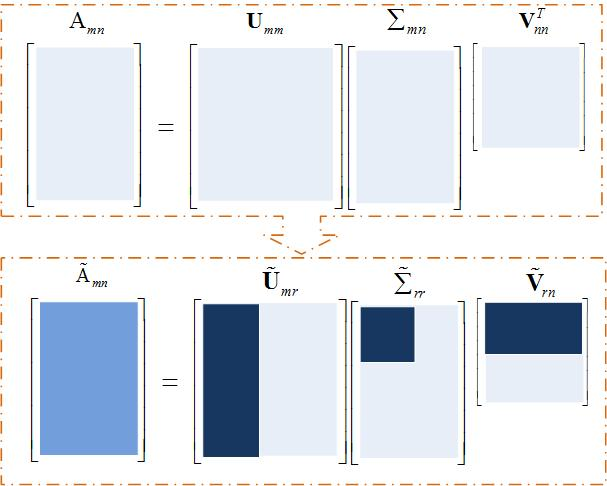
\includegraphics[width=0.6\textwidth]{SVDPCA.jpg}
\caption{SVD����ѹ��ʾ��ͼ��ȡǰ$r$������ֵ������$\widetilde{\bm{\Sigma}_{rr}}$�������Ӧ�����������( $\widetilde{\bm{U}_{mr}}$)�����������($\widetilde{\bm{V}_{nr}}$)�ľ���˵õ�����$\widetilde{\bm{A}_{mn}}$�����Խ���ԭ����$\bm{A}_{mm}$��ͨ������ǰ��ĺ��ٵ�����ֵ�Ϳ����Ժ�С����ʧ�ָ���ԭ����}
\label{fig:SVDPCA}
\end{figure}

ͼ\ref{fig:SVDPCA}ͼ�°벿����ʾ�ľ���ѹ�����̿�����ʽ��Ϊ
\begin{equation}\label{equ:SVDPCA}
  \widetilde{\bm{A}_{mn}}=\widetilde{\bm{U}_{mr}}\widetilde{\bm{\Sigma}_{rr}}\widetilde{\bm{V}_{rn}}^T
\end{equation}

��ʽ\ref{equ:SVDPCA}�����ҳ�$\widetilde{\bm{V}_{nr}}$���õ�һ��$m\times r$�׵ľ��������÷���$\widetilde{\bm{A}_{mr}}$���������ע�ⲻҪ������ʽ$\ref{equ:SVDPCA}$��$\widetilde{\bm{A}_{mn}}$������
\begin{equation}
\begin{split}
\widetilde{\bm{A}_{mr}}&=\widetilde{\bm{A}_{mn}}\widetilde{\bm{V}_{nr}}=\widetilde{\bm{U}_{mr}}\widetilde{\bm{\Sigma}_{rr}}\widetilde{\bm{V}_{rn}}^T\widetilde{\bm{V}_{nr}}\\
                        &=\widetilde{\bm{U}_{mr}}\widetilde{\bm{\Sigma}_{rr}}
\end{split}
\end{equation}
����$\widetilde{\bm{A}_{mr}}$��һ��$m\times r$�׵ľ�����ʵ���˶�ԭʼ����$\bm{A}_{mn}$���е�ѹ��������$r$���п��Կ����Ǵ�$\bm{A}_{mn}$��$n$��������ȡ������$r$���������������������ڵ�\ref{sec:PCA}����������PCA��ȡ�����ķ���������ͬ��֮�

�����˶Ծ��������ȡ�������ٽ��Ծ��������ȡ��������ʽ\ref{equ:SVDPCA}�������$\widetilde{\bm{U}_{mr}}^T$���õ�һ��$r\times n$�׵ľ��������÷���$\widetilde{\bm{A}_{rn}}$���������
\begin{equation}
\begin{split}
\widetilde{\bm{A}_{rn}}&=\widetilde{\bm{U}_{mr}}^T\widetilde{\bm{A}_{mn}}=\widetilde{\bm{U}_{mr}}^T\widetilde{\bm{U}_{mr}}\widetilde{\bm{\Sigma}_{rr}}\widetilde{\bm{V}_{rn}}^T\\
                        &=\widetilde{\bm{\Sigma}_{rr}}\widetilde{\bm{V}_{rn}}^T
\end{split}
\end{equation}
�������ǵõ���һ��$r\times n$�׵ľ���$\widetilde{\bm{A}_{rn}}$������ÿһ�ж���ԭʼ����$\bm{A}_{mn}$�������С�

���Կ����Ծ�����SVD����һ�Σ��ȿ�����ȡ�������ֿ�����ȡ���������ڵ�\ref{sec:PCA}����PCA�����ǶԾ�����ȡ�����������Ҫ�������������������Э����׶���Ҫ����dz�ʼ�����ת�õ�Э���\ref{fig:PCAvar}

\clearpage
\begin{lstlisting}[language=Python,title={sample.py},basicstyle=\scriptsize,captionpos=t]
import numpy
import scipy
import random
import matplotlib.pyplot as pyplot
import scipy.linalg as linalg
import scipy.stats as stats
def loaddata():
    dataset=[];   locset =[]
    center = numpy.array([2,2]);    direct = numpy.array([-1,1])
    gauss = stats.norm(0,0.6)
    direct = numpy.divide(numpy.array([-1,1]),linalg.norm(numpy.array([-1,1])))
    for i in range(50):
        bias = random.gauss(0,2)
        while numpy.abs(bias)>1.6:
            bias = random.gauss(0,0.4)
        loc =center +bias*center/linalg.norm(center)
        locset.append(loc)
        gausspdf = gauss.pdf(bias)
        label =random.random()-0.5
        dataset.append(loc+label*gausspdf*direct)
    return numpy.array(dataset),numpy.array(locset)
def plot(dataset,locset):
    pyplot.plot(dataset[:,0],dataset[:,1],'r^')
    locset[:,0] = locset[:,0]+0.3;locset[:,1]=locset[:,1]-0.3
    pyplot.plot(locset[:,0],locset[:,1],'k+')
    for i in range(dataset.shape[0]):
        pyplot.plot([locset[i,0],dataset[i,0]],[locset[i,1],dataset[i,1]],'y--')
    pyplot.annotate('',xytext=(1.6,1.6),xy=(3.0,3.0),arrowprops=dict(facecolor='black',width =3, shrink=0.01))
    pyplot.annotate('',xytext=(1.65,1.65),xy=(1.45,1.85),arrowprops=dict(facecolor='black',width =1, shrink=0.01))
    pyplot.text(1.5,1.9,'Noise',color="black",ha="center")
    pyplot.text(2.8,3,'Signal',color="black",ha="center")
    pyplot.xlim(0.5,3.5);    pyplot.ylim(0.5,3.5)
    pyplot.xlabel("x axis");    pyplot.ylabel("y axis")
    pyplot.show()
dataset,locset =loaddata()
plot(dataset,locset)
\end{lstlisting}
\clearpage

\begin{lstlisting}[language=Python,title={svd.py},basicstyle=\scriptsize,captionpos=t]
import numpy
import random
import matplotlib.pyplot as pyplot

data = numpy.array([[1,0.6,1,0,0.4],\
                    [2,1.7,2,0.2,0],\
                    [1,0,1,0.1,0],\
                    [3.2,4.8,5,0,0.4],\
                    [1,1,1.3,2,2],\
                    [0,0,0,3.2,3],\
                    [0,0,0,0.9,1]])
U,Sigma,VT=numpy.linalg.svd(data)
print U.shape,VT.shape,Sigma.shape
print Sigma
i=2
colomnclass=data.dot(VT[:i,:].T)
print colomnclass
rowclass = U[:,:i].T.dot(data)
print rowclass

pyplot.figure(1)
ax1=pyplot.subplot(211)
ax2=pyplot.subplot(212)
pyplot.sca(ax1)
pyplot.plot(colomnclass[:,0],colomnclass[:,1],'s')
pyplot.sca(ax2)
pyplot.plot(rowclass[0,:],rowclass[1,:],'^')
pyplot.show()
\end{lstlisting}

\begin{thebibliography}{9}
\bibitem{}{LeftNotEasy},{����ѧϰ�е���ѧ(5)-ǿ��ľ�������ֵ�ֽ�(SVD)����Ӧ��}, \url{http://www.cnblogs.com/LeftNotEasy/archive/2011/01/19/svd-and-applications.html}, 01/19 2011.
\bibitem{}{LeftNotEasy},{����ѧϰ�е���ѧ(4)-�����б������LDA��, ���ɷַ���(PCA)}, \url{http://www.cnblogs.com/LeftNotEasy/archive/2011/01/08/lda-and-pca-machine-learning.html}, 01/08 2011.
\bibitem{}{jerrylead},{���ɷַ�����Principal components analysis��-��󷽲����}, \url{http://www.cnblogs.com/jerrylead/archive/2011/04/18/2020209.html}, 04/18 2011.
\bibitem{}{260682605},{PCAԭ����Ӧ��}, \url{http://220.181.112.102/view/eecbe0110b4e767f5acfce8b.html}, 11/03 2012.
\bibitem{}{Vincent��},{����������LDA��}, \url{http://blog.csdn.net/chlele0105/article/details/13005527 }, 10/24 2013.
\bibitem{}{Linear discriminants analysis}, \url{http://research.cs.tamu.edu/prism/lectures/pr/pr_l10.pdf }.
\bibitem{}{Max Welling},{Fisher Linear Discriminant Analysis}, \url{http://www.ics.uci.edu/~welling/classnotes/papers_class/Fisher-LDA.pdf }
\bibitem{}{Vincent��},{���ɷַ�����Principal components analysis��}, \url{http://blog.csdn.net/chlele0105/article/details/13004499 }, 10/24 2013.
\bibitem{}{Vincent��},{Singular Value Decomposition (SVD) tutorial }, \url{http://web.mit.edu/be.400/www/SVD/Singular_Value_Decomposition.htm }, 10/24 2013.
\bibitem{}{We Recommend a Singular Value Decomposition}, \url{http://www.ams.org/samplings/feature-column/fcarc-svd }.

\bibitem{}{ccjou},{�����Q��ꇿ��������ǻ����C��}, \url{https://ccjou.wordpress.com/2011/02/09/%E5%AF%A6%E5%B0%8D%E7%A8%B1%E7%9F%A9%E9%99%A3%E5%8F%AF%E6%AD%A3%E4%BA%A4%E5%B0%8D%E8%A7%92%E5%8C%96%E7%9A%84%E8%AD%89%E6%98%8E/}, 02/09 2011.
\bibitem{}{iMetaSearch},{Latent Semantic Analysis (LSA) Tutorial },    \url{http://www.puffinwarellc.com/index.php/news-and-articles/articles/33-latent-semantic-analysis-tutorial.html?start=6}.
\end{thebibliography}






\newcommand{\mybayes}{Naive Bayes}%{Na\"{\i}ve Bayes}
\chapter{\mybayes}
���ر�Ҷ˹(\mybayes)���ǻ���{\bf ��Ҷ˹����}��{\bf ����������������}�ķ��ࡣ���ڸ�����ѵ�����ݼ�$\bm{T}$����������$\bm{x}=(x^{(1)},x^{(2)},\cdots,x^{(n)})$�����ǩ$y$��ɵĶ�$\langle \bm{x},c\rangle$ �ļ��ϣ������Ȼ�������������������ѧϰ����/��������ϸ��ʷֲ���Ȼ����ڴ�ģ�ͣ��Ը���������$\bm{x}$,���ñ�Ҷ˹���������������������$c$��\mybayes �����ص����ԭ����ʵ�ֶ��ܼ򵥣�����ѧϰ��ԤCE��Ч�ʶ��ܸߡ�
\section{\mybayes ��������}
����ռ�$\bm{\mathcal{X}}\subseteq \bm{R}^{n}$Ϊ$n$ά�����ļ��ϣ�����ռ�Ϊ����$K$��Ԫ�ص����Ǽ���$\bm{\mathcal{Y}}=\{c_1,c_2,\cdots,c_K\}$,��������������$\bm{x}\in\bm{\mathcal{X}}$,���Ϊ���ǩ(class label)$y\in \bm{\mathcal{Y}}$��$\bm{X}$�Ƕ���������ռ�$\bm{\mathcal{X}}$�ϵ��������,$Y$�Ƕ���������ռ�$\bm{\mathcal{Y}}$�ϵ����������$P(\bm{X},Y)$��$\bm{X}$��$Y$�����ϸ��ʷֲ���ѵ�����ݼ�
\begin{equation*}
  \bm{T}=\{\langle\bm{x}_1,y_1\rangle,\langle\bm{x}_2,y_2\rangle,\cdots,\langle\bm{x}_N,y_N\rangle\}
\end{equation*}
���Կ�����$P(\bm{X},Y)$����ͬ�ֲ�������

\mybayes ����ͨ��ѵ�����ݼ�ѧϰ�ո��ᵽ�����ϸ��ʷֲ�$P(\bm{X},Y)$����ʵ��ѧϰ������ֱ��ѧ������������ʷֲ����������ʷֲ��������ʽ�������£�

������ʷֲ�
\begin{equation}
\label{equ:priorpro}
  P(Y=c_k)\qquad,k=1,2,\cdots,K
\end{equation}
�������ʷֲ�
\begin{equation}
\label{equ:conpro}
  P(\bm{X}=\bm{x}|Y=c_k)=P(\bm{X}^{(1)}=\bm{x}^{(1)},\cdots,\bm{X}^{(n)}=\bm{x}^{(n)}|Y=c_k),\quad k=1,2,\cdots,K
\end{equation}

\mybayes ���������ʷֲ��������������Եļ��裬����һ����ǿ�ļ��裬\mybayes �������������أ��������������ǣ�
\begin{equation}
    \label{equ:duli}
    \begin{split}
  P(\bm{X}=\bm{x}|Y=c_k)    &=P(\bm{X}^{(1)}=\bm{x}^{(1)},\cdots,\bm{X}^{(n)}=\bm{x}^{(n)}|Y=c_k)\\
                            &=\prod_{j=1}^{n}P(\bm{X}^{(j)}=\bm{x}^{(j)}|Y=c_k)
  \end{split}
\end{equation}

\mybayes ������ʱ���Ը���������${\bm{x}}$,ͨ��ѧϰ����ģ�ͼ���������$P(Y=c_k|\bm{X})$�������������������Ϊ${\bm{x}}$�������������ʵļ�����ݱ�Ҷ˹�������У�
\begin{equation}
    \label{equ:nobayes}
  P(Y=c_k|\bm{X}=\bm{x})=\frac{P(\bm{X}=\bm{x}|Y=c_k)P(Y=c_k)}{\sum_{k=1}^{K}P(\bm{X}=\bm{x}|Y=c_k)P(Y=c_k)}
\end{equation}
��ʽ(\ref{equ:duli})����ʽ(\ref{equ:nobayes})��
\begin{equation}
    \label{equ:bayes1}
  P(Y=c_k|\bm{X}=\bm{x})=\frac{P(Y=c_k)\prod_{j=1}^{n}P(\bm{X}^{(j)}=\bm{x}^{(j)}|Y=c_k)}{\sum_{k=1}^{K}P(Y=c_k)\prod_{j=1}^{n}P(\bm{X}^{(j)}=\bm{x}^{(j)}|Y=c_k)},\quad k=1,2,\cdots,K
\end{equation}
���ǣ�\mybayes ���������Ա�ʾΪ
\begin{equation}
\label{equ:bayes2}
  y=f(\bm{x})=\arg\max_{c_k}\frac{P(Y=c_k)\prod_{j=1}^{n}P(\bm{X}^{(j)}=\bm{x}^{(j)}|Y=c_k)}{\sum_{k=1}^{K}P(Y=c_k)\prod_{j=1}^{n}P(\bm{X}^{(j)}=\bm{x}^{(j)}|Y=c_k)}
\end{equation}
ע�⵽ʽ(\ref{equ:bayes2})�ķ�ĸ����$P(\bm{x})$������һ����$c_k$�޹ص���������
\begin{equation}
\label{equ:bayes}
  y=\arg\max_{c_k}P(Y=c_k)\prod_{j=1}^{n}P(\bm{X}^{(j)}=\bm{x}^{(j)}|Y=c_k)
\end{equation}

���Ͼ���\mybayes �Ļ���ԭ��������һ������Ϳ���ʵ��һ���򵥵ı�Ҷ˹�������ˡ�
\section{������Ȼ���Ʋ���}
��ʽ(\ref{equ:bayes})��֪��\mybayes ��ѧϰ����Ҫ��ѵ����������$P(Y=c_k)$��$P(\bm{X}^{(j)}=\bm{x}^{(j)}|Y=c_k)$������Ӧ�ü�����Ȼ���Ʒ�������Ӧ�ĸ��ʡ������������\ref{tab:notations} ��ʾ
 \begin{table}[h]
  \centering
  %\scriptsize
  \caption{������������}
  \label{tab:notations}
  \begin{tabular}{ll}
    \\[-2mm]
    \hline
    \hline
    {\bf \small Symbol}&\qquad {\bf\small Meaning}\\
    \hline
    \vspace{1mm}\\[-3mm]

    $y_i$  &��$i$��������ǩ\\
    $c_k$   &��$k$��\\
    $\bm{x}_i$&       ��$i$������  \\
    $\bm{x}_i^{(j)}$& ��$i$�������ĵ�$j$������     \\
    $a_{jl}$ &��$j$����������ȡ�ĵ�$l$��ֵ\\
    $I$ &ָʾ����\\
    \hline
    \hline
  \end{tabular}
\end{table}

�������$P(Y=c_k)$�ļ�����Ȼ������
\begin{equation}
  P(Y=c_k)=\frac{\sum_{i=1}^{N}I\left(y_i=c_k\right)}{N},\quad k=1,2,\cdots,K
\end{equation}

���$j$������$x^{(j)}$���ܵ�ȡֵ����Ϊ$\{a_{j1},a_{j2},\cdots,a_{jS_j}\}$����������$P(X^{(j)}=a_{jl}|Y=c_k)$�ļ�����Ȼ������
\begin{equation}
  \begin{split}
    &P(X^{(j)}=a_{jl}|Y=c_k)=\frac{\sum_{i=1}^{N}I\left(x_i^{(j)}=a_{jl},y_i=c_k\right)}{\sum_{i=1}^{N}I\left(y_i=c_k\right)}\\
    &j=1,2,\cdots,n;l=1,2,\cdots,S_j;k=1,2,\cdots,K
  \end{split}
\end{equation}
\section{����������������յĹ�ϵ}
\mybayes ��������ʵ��$\bm{x}$���鵽����������(������ʾ���ʽ(\ref{equ:nobayes})��������������ʽ(\ref{equ:bayes})����)���������ǽ�Ҫ֤����һ�ڵ�``����������''�̺���``����������С��''��һָ��׼��

����ѡ��$0-1$��ʧ������
\begin{eqnarray*}
L(Y,f(\bm{X}))=
  \begin{cases}
    1,\quad &Y\neq f(\bm{X}) \\
    0,\quad&Y = f(\bm{X})
  \end{cases}
\end{eqnarray*}
ʽ��$f(\bm{X})$�Ƿ�����ߺ�������ʱ���������պ���Ϊ
\begin{equation*}
  R_{exp}(f)=E[L(Y,f(\bm{X}))]
\end{equation*}
�����Ƕ����Ϸֲ�$P(\bm{X},Y)$ȡ�ģ��ɴ˶���ʽ����һ���Ƶ����£�
\begin{equation*}
  \begin{split}
    R_{exp}(f)  &=E_{\bm{X},Y}[L(Y,f(\bm{X}))]\\
                &=\sum_{\bm{X}}\sum_{Y}L(Y,f(\bm{X}))P(\bm{X},Y)\\
                &=\sum_{\bm{X}}\sum_{k=1}^{K}L(c_k,f(\bm{X}))P(\bm{X},c_k)\\
                &=\sum_{\bm{X}}\sum_{k=1}^{K}L(c_k,f(\bm{X}))P(c_k|\bm{X})P(\bm{X})\\
                &=\sum_{\bm{X}}P(\bm{X})\sum_{k=1}^{K}L(c_k,f(\bm{X}))P(c_k|\bm{X})\\
                &=E_{X}\sum_{k=1}^{K}L(c_k,f(\bm{X}))P(c_k|\bm{X})
  \end{split}
\end{equation*}
���Կ��Խ��������պ���д��
\begin{equation}
    \label{equ:exp}
  R_{exp}(f)=E_{X}\sum_{k=1}^{K}L(c_k,f(\bm{X}))P(c_k|\bm{X})
\end{equation}
�۲�ʽ(\ref{equ:exp})�����Է��ֶ���ÿ��$\bm{x}$�����Ӧ�ķ��պ���$L(c_k,f(\bm{X}))P(c_k|\bm{X})$�Ƕ�������ġ�Ϊ��ʹ����������С�������Զ�$X=\bm{x}$�����С�����ɴ˵õ�
\begin{equation}
\label{equ:expost}
  \begin{split}
    f(\bm{x})   &=\arg\min_{y\in \mathcal{Y}}\sum_{k=1}^{K}L(c_k,y))P(c_k|\bm{X}=\bm{x})\\
                &=\arg\min_{y\in \mathcal{Y}}\sum_{k=1}^{K}P(y \neq c_k|\bm{X}=\bm{x})\\
                &=\arg\min_{y\in \mathcal{Y}}\sum_{k=1}^{K}(1-P(y = c_k|\bm{X}=\bm{x}))\\
                &=\arg\min_{y\in \mathcal{Y}}(1-P(y = c_k|\bm{X}=\bm{x}))\\
                &=\arg\max_{y\in \mathcal{Y}}P(y = c_k|\bm{X}=\bm{x})
  \end{split}
\end{equation}
��ʽ(\ref{equ:expost})����֪������������������С��׼������Ƶ�������������׼��
\begin{equation}
    \label{equ:expost2}
  f(\bm{x})=\arg\max_{c_k}P(c_k|\bm{X}=\bm{x})
\end{equation}
Ҳ����\mybayes �����õ�ԭ�������Կ���ʽ(\ref{equ:expost2})��ʽ(\ref{equ:bayes})�ǵ�Ч�ġ�
\section{���������任���������}
\mybayes ����һ������֮�������������ҵ���һ�������ģ�͵ȼ۵���ʽ���Ǿ������ǿ���ʹ���ϸ񵥵��任��$P(c|\bm{x})$�ͷ�����ֵ$t$ͬʱ�任�������������䡣��$T$���ϸ񵥵����������������������������������Ǽ�����ϸ񵥵��任�����⡣
\begin{equation*}
  \begin{split}
    P(c|\bm{x})>t &\iff T\left(P(c|\bm{x})\right)>T(t)\\
    P(c|\bm{x})>P(c|\bm{y}) &\iff T\left(P(c|\bm{x})\right)>T\left(P(c|\bm{y})\right)\\
    f(\bm{x})=\arg\max_{y\in \mathcal{Y}}P(y = c_k|\bm{X}=\bm{x}) &\iff \arg\max_{y\in \mathcal{Y}}T\left(P(y = c_k|\bm{X}=\bm{x})\right)
  \end{split}
\end{equation*}
���庯��ʽ(\ref{equ:1}),(\ref{equ:2})�ֱ�����ĺ����������ֲ�ͬ�ĵ��������任��
\begin{eqnarray}
  T_1(x)&= &\frac{x}{1-x} \quad 0 \leq x < 1 \label{equ:1}\\
  T_2(x)&= &\ln x \quad x>0 \label{equ:2}
\end{eqnarray}
��ʽ(\ref{equ:bayes1})(����$K=2$�������ǩֻ��$c_1,c_2$����)����ʽ(\ref{equ:1})�ı任($k=1$Ϊ����$k=2$ͬ$k=1$)��
\begin{equation}
\label{equ:trans1}
\begin{split}
T_1\left(P(Y=c_1|\bm{X}=\bm{x})\right)    &=\frac{P(Y=c_1|\bm{X}=\bm{x})}{1-P(Y=c_1|\bm{X}=\bm{x})}\\
                                        &=\frac{P(Y=c_1|\bm{X}=\bm{x})}{P(Y=c_2|\bm{X}=\bm{x})}\\
                                        &=\frac{P(c_1)}{P(c_2)}\frac{P(\bm{x}|c_1)}{P(\bm{x}|c_2)}\\
                                        &=\frac{P(c_1)}{P(c_2)}\prod_{i=1}^{n}\frac{P(x_i|c_1)}{P(x_i|c_2)}
\end{split}
\end{equation}
��ʽ(\ref{equ:trans1})����ʽ(\ref{equ:2})�ı任,�ɵõ���һ���������
\begin{equation}
\label{equ:trans2}
  \begin{split}
    T_2\left(T_1\left(P(Y=c_1|\bm{X}=\bm{x})\right)\right) =\ln{\frac{P(c_1)}{P(c_2)}}+\sum_{i=1}^{n}\ln \frac{P(x_i|c_1)}{P(x_i|c_2)}
  \end{split}
\end{equation}
���Ƕ���$w_0=\ln{\frac{P(c_1)}{P(c_2)}}$��$w_i(x_i)=\ln \frac{P(x_i|c_1)}{P(x_i|c_2)}$�������庯��
\begin{equation}
\label{equ:3}
  T(x)=T_2\left(T_1\left(x\right)\right)
\end{equation}
��ʵʽ(\ref{equ:3})Ҳ��һ�����������任��������ʽ(\ref{equ:trans2})����дΪ��
\begin{equation}
  T\left(P(Y=c_1|\bm{X}=\bm{x})\right)=w_0+\sum_{i=1}^{n}w_i(x_i)
\end{equation}

��������Ƶ�Ϊ���������Ƕ�����������
\begin{equation}
\label{equ:weight}
  S(c_1,\bm{x})=w_0+\sum_{i=1}^{n}w_i(x_i)
\end{equation}
��ʾ����$\bm{x}$�����$c_1$�Ĵ�֣���Ȼ$\bm{x}$�����$c_2$�Ĵ��������$S(c_2,\bm{x})$������ȶ���,���û���ر�˵��������һ�ɶ�$S(c_1,\bm{x})$�������ۡ�����$S(c_1,\bm{x})$��$S(c_2,\bm{x})$�������֣����ǾͿ��԰�$\bm{x}$���鵽���ָߵ�������ʵ���˷�������Ŀ�ġ�

�ٿ�����ļ����任����������֪����ֵ$S=w_0+\sum_{i=1}^{n}w_i(x_i)$��ֱ����$P(c|\bm{x})$�Ĺ���ֵ��������ģ�����\mybayes ģ����ʵ���Ƕ�ԭʼ$x_i$�ı任�ļ���͡�

���ÿ������������ɢ�Ļ����ǽ����������ָ�ΪС�ĵ�Ԫ����ɢ����ʽ(\ref{equ:weight})����ʽ���ر�򵥡��DZ���$x_i$ȡ���$k_i$ ����Ԫ��ֵ��$x_i^{(k_i)}$,��ô$w_i\left(x_i^{(k_i)}\right)$����``�����ݶ�''֮�ȵĶ������������$c_1$�ĵ��ڱ���$x_i$��ȡֵ����ĵ�$k_i$����Ԫ�ķݶ�������$c_2$�ĵ��ڱ���$x_i$��ȡֵ����ĵ�$k_i$����Ԫ�ķݶ��ʱ�����$w_i\left(x_i^{(k_i)}\right)$ ��ΪȨ�أ�����$i$���������ܷ�ֵ�Ĺ��ף����ߵ�$i$������Ϊ������$\bm{x}$���鵽���$c_1$�ṩ��֤�ݡ�������Щ֤��Ȩ�أ�����ʶ�����Щ���������ж���һ�ض����������������Ҫ�ġ�
\section{������������׼���չ}
��$1$���ᵽ\mybayes ���������ʷֲ��������������Եļ��裬����һ�������ص㽲���ö����Լ���������Լ����Ƕ���׶�����ĸ��ƴ�ʩ��
\subsection{Ϊʲô�����Լ������}
\subsubsection{���͸��Ӷ�}
ʽ(\ref{equ:conpro})��������������ʷֲ�$P(\bm{X}^{(1)}=\bm{x}^{(1)},\cdots,\bm{X}^{(n)}=\bm{x}^{(n)}|Y=c_k)$��ָ���������IJ������ٶ�$x^{(j)}$��ȡֵ��$S_j$����$j=1,2,\cdots,n$����$\bm{x}$���ܵ������$\prod_{j=1}^{n}S_j$�֣��ּ���$Y$���ܵ�ȡֵ��$K$ ���������ô�����ĸ���Ϊ$K\prod_{j=1}^{n}S_j$������������еIJ������й��ƣ�����Ҫ������������㹻���ѵ�����ݼ����������ǻ�����$\bm{X}$��ά�ȵ����Ӷ���ը��������ά����ը������������˾�ɥ���������е��о��߶�ѡ������â��

�����������������Լ���󣬼�
\begin{equation*}
P(\bm{X}^{(1)}=\bm{x}^{(1)},\cdots,\bm{X}^{(n)}=\bm{x}^{(n)}|Y=c_k)=\prod_{j=1}^{n}P(\bm{X}^{(j)}=\bm{x}^{(j)}|Y=c_k)
\end{equation*}
�����Ӷȷ�����Ϸ���Եظ��ƣ������ĸ�������������������������$K\sum_{j=1}^{n}S_j$�����ָ���ʹ��Ҷ˹��������ʵ���ԡ�
\subsubsection{ѵ����������Ԥ����}
���ݼ�ͨ�������ڽ�����ѧǰ�Ѿ�������һ������ѡ����̣��������Իع��еı���ѡ�񷽷����ù��̽��߶���ر����޳���ʣ�µı���֮����ܽӽ��ڶ�����ϵ��
\subsubsection{���벻ңԶ}
�����Լ�����ܻᵼ�²�ĸ��ʹ��ƻ���$\frac{P(c_1|\bm{x})}{c_2|\bm{x}}$���ʹ��ƣ����Ⲣ����ζ�Ź��Ƶõ��ľ��������ʵ�ľ����������Զ��
\subsubsection{�����Է�����}
\mybayes �������ľ�������Ծ��и��ӵķ�������״����Ȼ������(ʽ(\ref{equ:weight}))����$w_i(x_i)$�����Եģ�������ԭʼ����$x_i$�Ǹ߶ȵķ����ԣ�����������ϳ��dz����ӵ����档
\subsection{����ϵ��������}
���Լ�Ķ����Լ��谵ʾ��\mybayes �������о����Եģ��Ͼ���ʵ�������м����б������������Ρ����������Ǵ�``ƫ��-����''����ԭ���ĽǶ�˵��ģ�ͼ����ƫ���Ӱ�첢��������ϵ������������Ӱ�졣
\subsubsection{``ƫ��-����''����ԭ��}
��ͳ��ѧ�������ھ�����``ƫ��-����''����ԭ��(bias-variance tradeoff)����ͬʱ�Ż��е�ʦѧϰ�㷨������ģ�Ͷ�ѵ�����ݼ�֮������ݼ����罻����֤�е�CE�Լ����ķ���������������
\begin{itemize}
  \item {\bf ƫ��}(bias)��Դ�ڴ����ģ�ͼ���
  \item {\bf ����}(variance)��Դ�ڶ�ѵ�����ݵIJ�����������
\end{itemize}
\begin{figure}[!ht]
\centering
\subfigure[Function and noisy data]{
\label{fig:a}
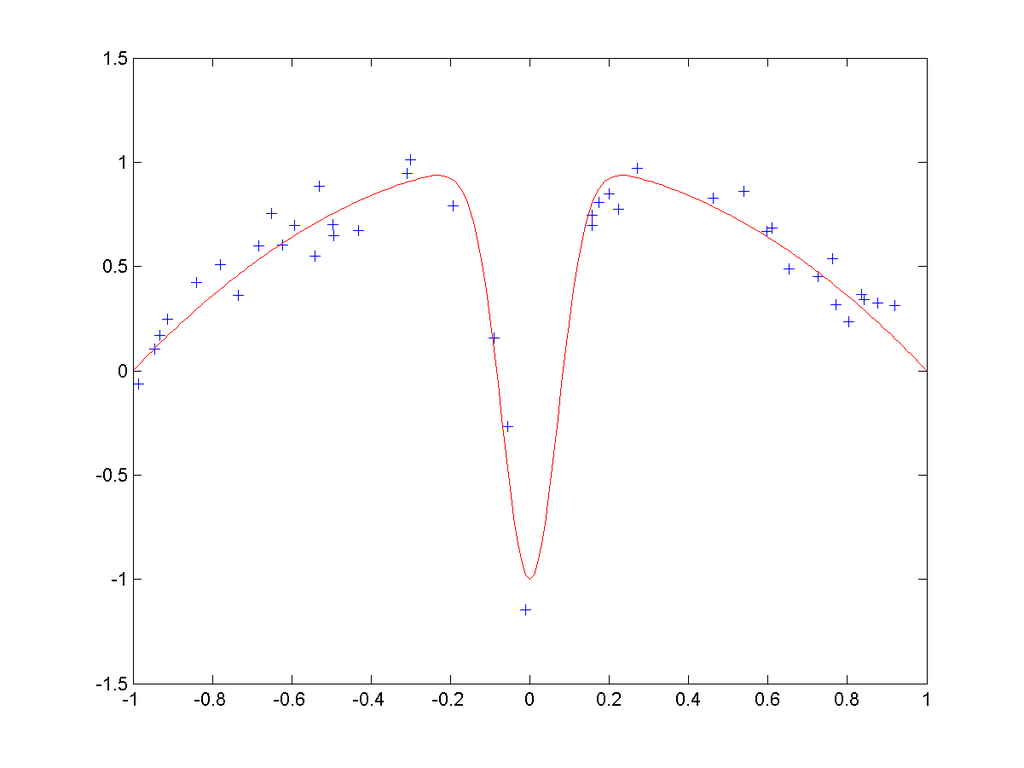
\includegraphics[width=0.4\textwidth]{bias1.png}}
\hspace{0.5in}
\subfigure[$\sigma$=5]{
\label{fig:b}
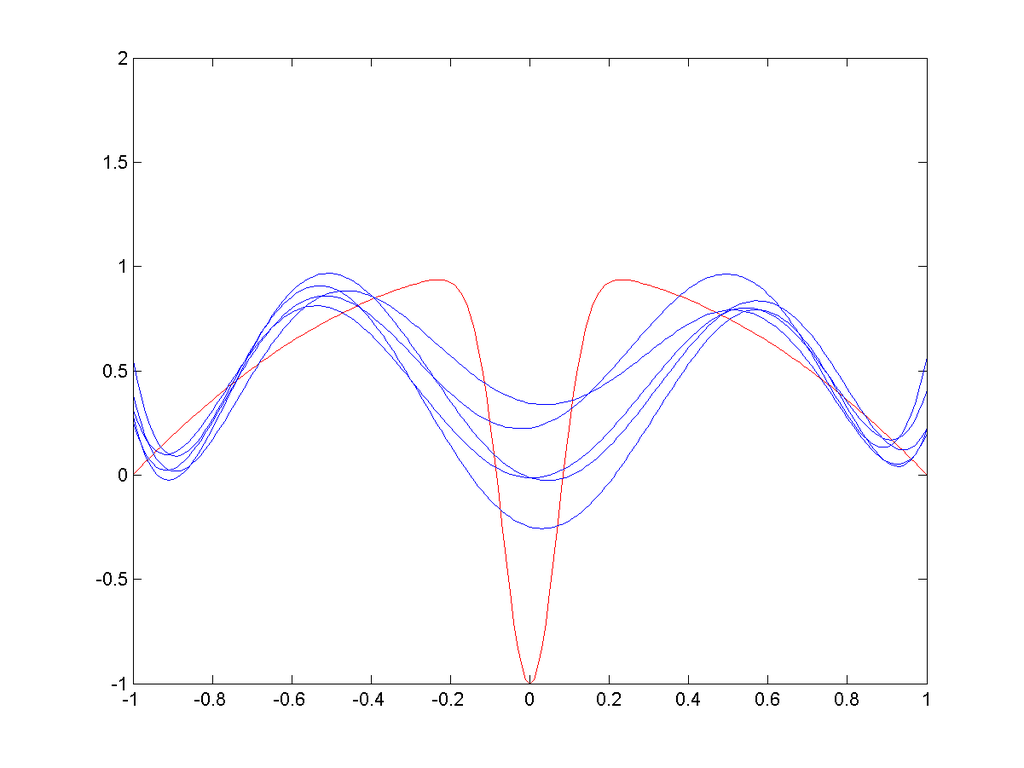
\includegraphics[width=0.4\textwidth]{bias2.png}}

\subfigure[$\sigma$=1]{
\label{fig:c}
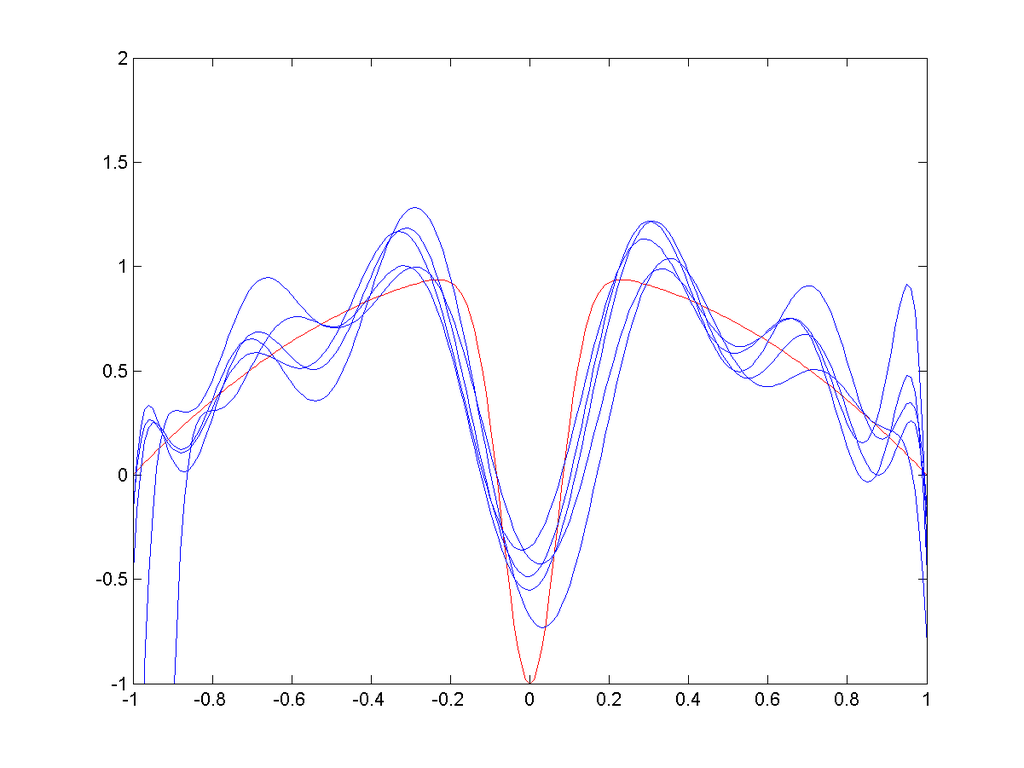
\includegraphics[width=0.4\textwidth]{bias3.png}}
\hspace{0.5in}
\subfigure[$\sigma$=0.1]{
\label{fig:d}
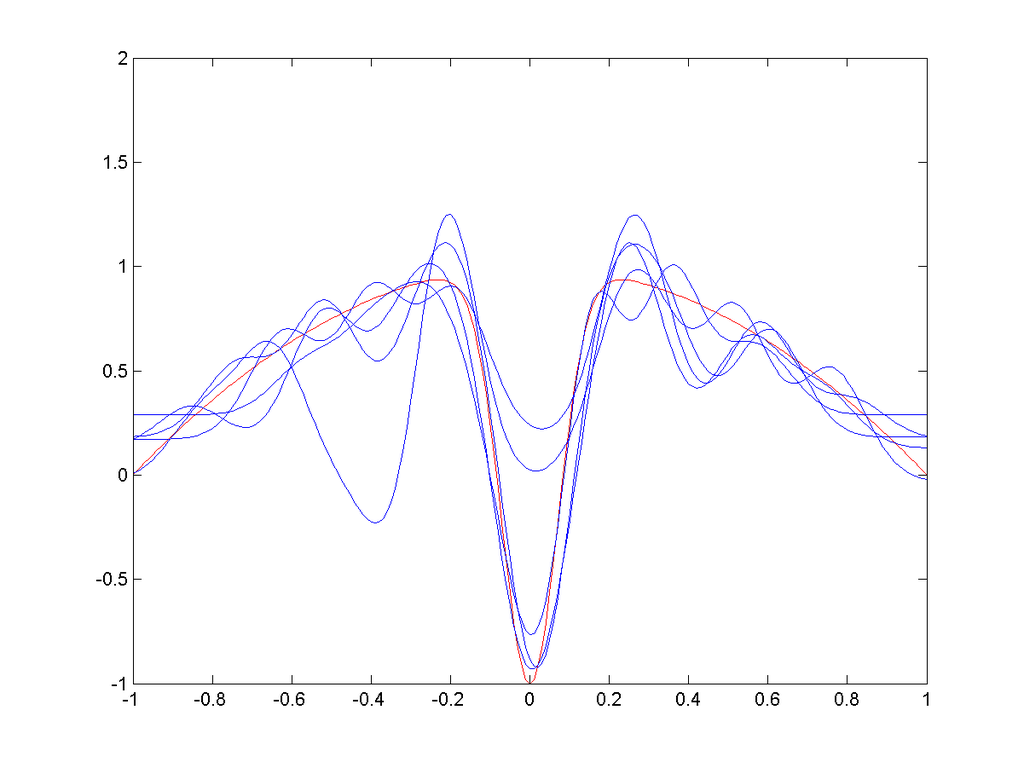
\includegraphics[width=0.4\textwidth]{bias4.png}}
\caption{A function (red) is approximated using RBF (blue). Several trials are shown in each graph. For each trial, a few noisy data points are provided as training set. For a big $\sigma$ (image \ref{fig:b}) the bias is high(i.e.the RBFs cannot fully approximate the function,especially the central dip), but the variance between different trials is low. As $\sigma$ decreases (image \ref{fig:c} and \ref{fig:c}) the bias decreases(i.e.the blue curves more closely approximate the red). However, depending on the noise in different trials the variance between trials increases. In image\ref{fig:d} the approximated values for x=0 varies wildly depending on where the data points were located.}
\label{fig:bias_variance}
\end{figure}
ͼ\ref{fig:bias_variance}�þ���������ƽ�������ݵĹ��̡����Կ�������ģ�ͼ���ĸ��Ӷȵ����(�������������չ�ٶ�$\sigma$�ļ�С)��ģ�Ͷ���Ӧ��ѵ�����ݼ���ƫ��(bias)���ͣ����Dz�ͬѵ�����ݼ�ѵ��������ģ��֮��ķ���(variance)ȴ���ӣ���ͼ\ref{fig:bias_variance_show}��������ģ�ͼ���ĸ��Ӷ�Ҫȡ���У������`` ƫ��- ����''����ԭ����
\begin{figure}[h]
    \centering
  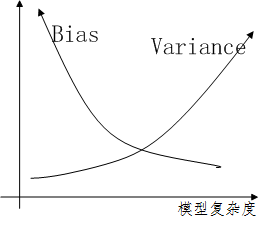
\includegraphics{bias5.png}
  \caption{``����-ƫ��''����ʾ��ͼ,Ϊ��ʵ�ַ����ƫ����ߵľ��⣬��Ҫ��ģ�ͼ���ĸ��Ӷ�ȡ���У���ģ��̫�����˻�̫���˶�����ȡ}
  \label{fig:bias_variance_show}
\end{figure}

˳����һ�£�``ƫ��-����''�ֽⷽ�����㷨�ķ�����������ֽ��Ϊ���ƫ��Ͳв�(����)�������ֽ��еķ�����``ƫ��-����''����ԭ�����ڸ����е�ʦѧϰ�㷨: classification��regression ��and structured output learning����Ҳ���ڽ�������ʽ�㷨����Ч�ԡ�

\subsubsection{����ϵ��}
�ڶ�ΪʲôҪ������֮���������Լ��������������֪����$n$��һԪ�����༭�ֲ��ĸ�����ԶԶС��һ��$n$Ԫ���������Ϸֲ�������ζ�ţ�Ϊ�˴ﵽͬ����ģ�;��ȣ�����ģ�ͱȷǶ���ģ����Ҫ���ٵ����ݵ㡣���仰˵�������ģ������Ϊ�������ж����ԣ���ô���ڸ������������Ĺ��Ƶķ���ͱȽ�С����Ȼ������ü�����ʵ�ʲ������ͻ���ƫ������ķ��ա���Ҳ��``ƫ��-����''����ԭ�������֡�

Ϊ�˼��ٶ����Լ��������ƫ����գ�\mybayes ��һ���򵥵����������������Ϊ��������������Ĺ������ƣ���������һ�ּ�������\raisebox{0.5mm}{------}���еı�����ȫ��أ�����������£����еı���������ͬ�ı߼ʷֲ��Ҹñ߼ʷֲ������Ϸֲ���ȣ������ֵΪ$r$ �� ��\mybayes ���ƣ����������Լ����µ��������ʣ�
\begin{equation}
\label{equ:bayr}
  \frac{P(c_1|\bm{x})}{P(c_2|\bm{x})}=\frac{P(c_1)}{P(c_2)}\prod_{i=1}^{n}\frac{P(x_i|c_1)}{P(x_i|c_2)}=r^n
\end{equation}
��ʵ��ʵ�����Ʊ�(odd ratio)�ǣ�
\begin{equation}
\label{equ:realr}
 \frac{P(c_1|\bm{x})}{P(c_2|\bm{x})}=\frac{P(c_1)}{P(c_2)}\frac{P(\bm{x}|c_1)}{P(\bm{x}|c_2)}=r
\end{equation}

ͨ����ʽ(\ref{equ:bayr}),(\ref{equ:realr})�ĶԱȣ�����ԵĴ��ڻ�ʹ\mybayes �߹���$r>1$����͹���$r<1$�����Ʊ�$\frac{P(c_1|\bm{x})}{P(c_2|\bm{x})}$��

����һ������Եõ�һ���޸�\mybayes ���ƵIJ��ԣ����Ƕ�$\frac{P(x_i|c_1)}{P(x_i|c_2)}$ȡһ��С��$1$���ݣ��������������ʵ�����Ʊ�������£������γ�һ�ָ�����\mybayes ���ƣ�
\begin{equation}
\label{equ:baybetter}
  \frac{P(c_1|\bm{x})}{P(c_2|\bm{x})}=\frac{P(c_1)}{P(c_2)}\prod_{i=1}^{n}\left(\frac{P(x_i|c_1)}{P(x_i|c_2)}\right)^{\beta}\quad,\beta\leq 1
\end{equation}

ͨ��Ҫ����$\beta$���п��ܵ�ȡֵ���ý�����֤�ȷ�����ÿ��ȡֵ��Ӧ��ģ�ͽ������������ȷ���ܲ�����õ�ԤCE�����$\beta$ֵ�������ʽ(\ref{equ:weight})�������൱�ڸ�$w_i\left(x_i\right)$����һ������ϵ����


\section{������˹ƽ��}
�ü�����Ȼ���ƿ��ܻ����Ҫ���Ƶĸ���ֵΪ0���������ʱ��Ӱ�쵽������ʵļ�����������ʽ(\ref{equ:bayes1})����д���£�������ֻҪ��һ��Ϊ0��������ʾ�Ϊ0��������������ȡֵ���٣�����Ȼ�Dz���ƽ�ġ�
\begin{equation*}
  P(Y=c_k|\bm{X}=\bm{x})=\frac{P(Y=c_k)\prod_{j=1}^{n}P(\bm{X}^{(j)}=\bm{x}^{(j)}|Y=c_k)}{P(\bm{X})}
\end{equation*}
����ʽ�����Dz��ÿ���$P(\bm{X}=0$�������ֻ��Ҫ�跨ʹ��������$P(\bm{X}^{(j)}=\bm{x}^{(j)}|Y=c_k)$ ���������$P(c_k)$������ʽ�Ӳ�Ϊ$0$�Ϳ����ˣ��������ֱ����ۡ�


��������������(���������ñ�\ref{tab:notations}����ı���)

\subsection{�����������}
\begin{enumerate}
\item Ҫ�����ı���ʽ:
\begin{equation}
  P(Y=c_k)=\frac{\sum_{i=1}^{N}I\left(y_i=c_k\right)}{N},\quad k=1,2,\cdots,K
\end{equation}

\item ��������Ŀ��:
\begin{equation}
  P(Y=c_k)>0
\end{equation}
\item �����ƻ�������:
\begin{equation}
  \sum_{k=1}^{K}P(Y=c_k)=1
\end{equation}
\end{enumerate}
����Ȼ�أ����ǵ��������Ϊ
\begin{equation}
  P(Y=c_k)=\frac{\sum_{i=1}^{N}I\left(y_i=c_k\right)+\lambda_1}{N+K\lambda_1}\qquad \lambda_1>0
\end{equation}
\subsection{������������}
\begin{enumerate}
\item Ҫ�����ı���ʽ:
\begin{equation}
  P(X^{(j)}=a_{jl}|Y=c_k)=\frac{\sum_{i=1}^{N}I\left(x_i^{(j)}=a_{jl},y_i=c_k\right)}{\sum_{i=1}^{N}I\left(y_i=c_k\right)} \quad j=1,2,\cdots,n;l=1,2,\cdots,S_j;k=1,2,\cdots,K
\end{equation}

\item ��������Ŀ��:
\begin{equation}
  P(X^{(j)}=a_{jl}|Y=c_k)>0
\end{equation}
\item �����ƻ�������:
\begin{equation}
  \sum_{l=1}^{S_j}P(X^{(j)}=a_{jl}|Y=c_k)=1
\end{equation}
\end{enumerate}

����Ȼ�أ����ǵ��������Ϊ
\begin{equation}
  P(X^{(j)}=a_{jl}|Y=c_k)=\frac{\sum_{i=1}^{N}I\left(x_i^{(j)}=a_{jl},y_i=c_k\right)+\lambda_2}{\sum_{i=1}^{N}I\left(y_i=c_k\right)+S_j\lambda_2}\qquad \lambda_2>0
\end{equation}

$\lambda_1$��$\lambda_2$��ȡֵ��������ȫ����ģ����Զ��߿������Ҳ���Բ���ȡ�һ��ȡ$\lambda_1=\lambda_2=1$����ʱ��Ϊ������˹ƽ��(Laplace smoothing)��
\begin{thebibliography}{9}
\bibitem{lihang}
  �,
  \emph{ͳ��ѧϰ����}.
  �廪��ѧ������, ����,
  2014.
  \bibitem{Xindong}
  {Xindong Wu,Vipin Kumar},
  \emph{The Top Ten Algorithms in Data Mining}.
  CRC press, Taylor$\&$ Francis,
  2009.
\bibitem{bl}{leftnoteasy},{���Իع�,ƫ���뷽��Ȩ��}, \url{http://www.cnblogs.com/LeftNotEasy/archive/2010/12/19/mathmatic_in_machine_learning_2_regression_and_bias_variance_trade_off.html}, 12/19 2010.
\bibitem{bl}Bias�Cvariance tradeoff, \url{http://en.wikipedia.org/wiki/Bias-variance_tradeoff}, 12/19 2010.
\bibitem{lihang}
  ���,
  \emph{��ѧ֮��}-������ ͳ��ѧϰ����.
  �����ʵ������, ����,
  2013.
\end{thebibliography}




\chapter{PageRank�㷨}
\indent Google����``��ҳ����PageRank��''��``ҳ�����''���ּ�����ȷ�����������뾫ȷ�ʡ���νPageRank�����ǻ���������������ӽṹ������ҳ�����ӹ�ȣ�Link Popularity����������ҳ��Ҫ�ԡ���``ҳ�����''��ҳ������Ƿ���ֹؼ��ʡ���ҳ�ڹؼ��ʳ��ֵ�Ƶ�ʣ�keyword density�����ؼ��ʳ�����ʲôλ�õȣ���ȷ����Щ��ҳ������ִ�е�����������ء������ص㽲��ǰ�ߵ���ѧ���ơ�
\section{PageRank�㷨}
\indent ��ͳ���������ڻ������������ص㣺
\begin{enumerate}
  \item ���������������С\raisebox{0.5mm}{------}����һ���ֵ���¼����ͨ��ֻ��һ�������һ��ͼ�����¼�IJ��ظ�ͼ��ͨ����������ʮ���֣�һ���̵����Ʒͨ�������������֡�
  \item ��������������õķ��������\raisebox{0.5mm}{------}�����ֵ�����ְ�ƴ������ͼ������ͼ�鰴������࣬�̵������Ʒ��Ʒ�ֻ���;����ȵȡ�
  \item ����������ظ��Ƚϵ�\raisebox{0.5mm}{------}�����ֵ����ͬ����ͨ����������ʮ����ͼ������ͬ��ͼ����̵����ͬ����Ʒͨ��Ҳ��������ʮ�֡�
\end{enumerate}

\indent ���ڻ�����������ǰ�����ص㣬���Էֱ�ͨ�����ӷ��������������ʹ洢�ռ���ֶ�������������ڵ������ص㣬��ֻ�����Ⱦ�֪�������������Ҫ�Ե����򣬲���������ǰ�Ľ������չʾ���û���

\indent ÿ����ҳ�������Dz��ܿ���ҳ�Լ������Ƶģ� ����һ��������ҳ���۰ѹؼ����ظ����ٴΣ� ����Ȼ��������ҳ���û��������ùؼ���ʱ����ҳ��������Ȼ��Ҫ����ġ�

\indent ѧ��������ѧ��������Ҫ�Ե�ͨ�÷����� �Ǿ��ǿ����ĵ����ô������ڻ������ϣ� �����ĵ����������Ƶ�����Ȼ����ҳ�����ӣ���ôͨ���о���ҳ����໥������ȷ���������Ҳ��һ��˼·��ʵ���ϣ�PageRankҲ����ô���ġ� �����˵��һ����ҳ��������ҳ���ӵ�Խ�࣬ ���������Ӧ��Խ��ǰ�� ������ˣ�һ����ҳԽ�DZ�����ǰ����ҳ�����ӣ� ���������ҲӦ��Խ��ǰ�� ��һ��������Ҳ�Dz��Զ����ģ� �ͺñ�һƪ���ı�ŵ���������������ã� ��ȻҪ�ȱ���ͨ�о��������ø�˵�����ֵ��

\indent �������Dz���������صĸ��
\begin{enumerate}
  \item ��ҳ$i$������(in-links)����Щָ����ҳ$i$��������������ҳ�ij����ӣ�ͨ��������������ͬһվ������ҳ�ij����ӡ�
  \item ��ҳ$i$�ij���(out-links)����Щ����ҳ$i$ָ��������ҳ�ij����ӣ�ͨ��������ָ��ͬһվ������ҳ�ij����ӡ�
\end{enumerate}

\indent ǰ����������õĽǶȲ�����PageRank��˼�룬�������Ǵ���������(rank prestige)�ĽǶȽ��н�һ��������
\begin{enumerate}
  \item ��һ����ҳָ����һ��ҳ�ij�������PageRankֵ������ʽ���ݣ���ҳ��PageRankֵ����ָ���������е���ҳ�����ݹ�����PageRankֵ�ܺ;����ġ���������ҳ$i$������Խ�࣬����PageRankֵ���ܾ�Խ�ߣ����õ�������Ҳ��Խ�ߡ�
  \item һ����ҳָ����������ҳ����ô�����ݵ�����ֵ�ͻᱻ����ָ��Ķ����ҳ������Ҳ����˵����ʹ��ҳ$i$��һ��PageRankֵ�ܸߵ���ҳ$j$��ָ�������ҳ$j$�ij����dz��࣬��ҳ$i$����ҳ$j$�õ�������ֵ������ϡ��Ҳ��С��
\end{enumerate}
\indent ���ǿ��԰�Web�����һ������ͼ$G=(V,E)$,����$V$��ͼ�Ľڵ㼯��(һ���ڵ��Ӧһ����ҳ),$E$��ͼ������߼���(����߶�Ӧ������)����Web�ϵ���ҳ����Ϊ$n$(����$n=\mid\negthickspace V\negthickspace\mid$)������˼�������ʽ��Ϊ��
\begin{equation*}
  P(i)=\sum_{(j,i)\in E}\frac{P(j)}{O_j}
\end{equation*}
\indent ����$P(i)$��ʾ��ҳ$i$��PageRankֵ��$O_j$����ҳ$j$������������$(j,i)\in E$��ʾ������ҳ$j$ָ����ҳ$i$�ij����ӡ�����ѧ�Ĺ۵㿴�ʹ���һ������$n$��δ֪�������Է����飬������һ����������ʾ��������һ�����ŵ�Լ������������$\bm{P}$��ʾ$n$����ҳ�ĵ�PageRank ֵ�����£�
\begin{equation*}
  \bm{P}=\left(P(1),P(2),\cdots,P(n)\right)^T
\end{equation*}
���þ���A��ʾ����ͼ���ڽӾ��󣬲������¹���Ϊÿ������߸�ֵ��
\begin{eqnarray*}
\bm{A}_{ij}=
  \begin{cases}
    \frac{1}{O_i}\!&\mathrm{if}(i,j)\in E \\
    0\!&\mathrm{else}
  \end{cases}
\end{eqnarray*}
����������������ӽṹͼ
\begin{figure}[h]
    \centering
    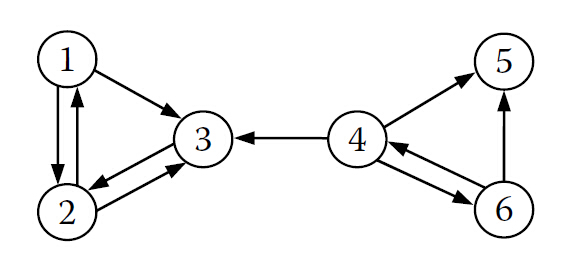
\includegraphics[width=0.5\textwidth]{network.jpg}
    \caption{����ij�����ͼ������}
    \label{fig:network}
\end{figure}
���Ӧ���ڽӾ���$\bm{A}$���£�\\
\begin{center}$\bm{A}$=$\begin{pmatrix}
0 & \frac{1}{2} & \frac{1}{2}   &0  &0  &0 \\
\frac{1}{2} & 0 & \frac{1}{2}   &0  &0  &0 \\
0 & 1 & 0 &0  &0  &0 \\
0 & 0 & \frac{1}{3}   &0  &\frac{1}{3}  &\frac{1}{3} \\
0 & 0 & 0   &0  &0  &0 \\
0 & 0 & 0   &\frac{1}{2}  &\frac{1}{2} &0
\end{pmatrix}$ \end{center}

\indent ���ǿ��Եõ����·����飺
\begin{equation}
  \bm{P}=\bm{A}^T\bm{P}
\end{equation}
\indent ���ǵ������������֪����$\bm{A}$��������,�������$\bm{P}$���ٿ������飬����$\bm{P}$��ѭ������ģ����Կ������������ݵ����������$\bm{P}$��
���Ƕ�����Ը�����ֵ$\bm{P}_0$������$\bm{P}_n$�Ǿ�����$n$�ε����õ���$\bm{P}$ֵ���������ʽ�����£�
\begin{equation}
  \begin{split}
    \bm{P}_{n+1}=\bm{A}^T\bm{P}_n\qquad,n=0,1,\cdots,\infty,\mathrm{given}~ \bm{P}_0
  \end{split}
\end{equation}
���㹫ʽ(1)������Ľ�$\bm{P}^{*}$����$\lim\limits_{n\rightarrow \infty}\bm{P}_{n}$��
\\ \indent ��Ȼ,Ҳ�����������Ʒ���(Markov chain)���н�ģ����ʱ $\bm{P}_{n}$ �Ϳ��Կ�����Markov chain��һ��״̬(state),$\bm{A}$ ���Ա�ʾ״̬ת�ƾ���(state transition matrix), �����Ϳ���ת���������Ʒ����ı����Ժͼ��޷ֲ����⡣
\\ \indent ����������Ҫ������������ǣ�
\begin{enumerate}
  \item $\lim\limits_{n\rightarrow \infty}\bm{P}_{n}$�Ƿ���ڣ�
  \item ������޴��ڣ����Ƿ���$\bm{P}_0$��ѡȡ�޹أ�
  \item ������޴��ڣ�������$\bm{P}_0$��ѡȡ�޹أ�����Ϊ��ҳ����������Ƿ���ĺ�����
\end{enumerate}

\indent �������������Ĵ𰸶��ǿ϶���,��ô��ҳ��������������ˡ���֮������ֻ��һ������Ĵ��Ƿ񶨵ģ���ҳ��������Ҳ�Ͳ������ǵõ�������������ôʵ�ʴ������?���ź�,�Ǻ�һ�֣�������������Ĵ�ȫ���Ƿ񶨵ġ� �������һЩ�򵥵����ӿ������ȷ�˵�� ��ֻ���������໥������ҳ�������ͻ������ϣ� ���$P_0=\left(1,0\right)^T$�����޾Ͳ����� ,��Ϊ���ʷֲ�����$\left(1,0\right)^T$��$\left(0,1\right)^T$֮�������񵴡������ڼ���������ͨ (����������) ����Ļ��������ʹ���ޡ���������ڡ��� ��$P_0$��ѡȡ�йأ���Ϊ��$P_0$ ѡ�ڲ�ͬ��������Ȼ�ᵼ�²�ͬ���ޡ� ���ڼ��޴��ڣ�������$P_0$��ѡȡ�޹�ʱ����Ϊ��ҳ����������Ƿ���ĺ��������⣬��Ȼ������ѧ���⣬��ȴҲ�Ƿ񶨵ģ� ��Ϊ�κ�һ��``������ҳ''������ڶ�һ���� ��������ҳ�ĸ��� �����ա� ���Լ����϶���������``�ͷ�''������Ȼ�Dz������ġ����ֲ�����ЧӦ����������� ��������һ����ͨ�����õĻ������ϣ� ����ֻ��һ�� `` ������ҳ''�� Ҳ����ʹ��������������ҳ����ʧЧ��
\\indent �ڽ�һ������֮ǰ���������뼸�����
\begin{itemize}
  \item ������(Positive matrix):ÿ������Ԫ������0�ľ���ÿ��Ԫ�ض����ڵ���0�ľ����ǷǸ�����(Nonnegative matrix).
  \item ����(Primitive matrix)���ؾ�����ָ������ij������Ϊ������(Positive matrix)�ľ�����$\bm{A}$Ϊһ��$n\times n$�ķ���, �������������$k$ ʹ�þ���
      \begin{equation*}
        \bm{A}^k>0
      \end{equation*}
      ��ô, �ƾ���$\bm{A}$Ϊ�ؾ���
  \item �������(stochastic matrix)����������ֽи��ʾ���probability matrix����ת�ƾ���transition matrix���������Ʒ����Markov matrix���ȡ��������ͨ����ʾ���������(left stochastic matrix)�����������$\bm{A}_{n\times n}$Ϊ�����������������������������
      \begin{equation*}
        \begin{split}
        \mathrm{suppose~}&a_{i,j}  \mathrm{~is~the~element~from~}\bm{A} \mathrm{~at~row~} i ,\mathrm{~colomn~} j,\mathrm{then~we~have~}\\
          &\forall i=1..n, j=1..n,a_{i,j}\geq 0\\
          &\forall i=1..n,\sum_{j=1}^{n}a_{ij}=1\\
        \end{split}
      \end{equation*}
      ����������ת�ó�Ϊ���������(right stochastic matrix)��
  \item ����Լ����irreducible matrix��������$\bm{A}$�Dz���Լ�ĵ��ҽ��������$\bm{A}$��Ӧ������ͼ��{\bf ǿ��ͨ}�ġ�����ͼ$G=(V,E)$��ǿ��ͨ�ĵ��ҽ�����ÿһ�ڵ��$u,v\in V$�����ڴ�$u$��$v$��·����Ҳ����˵�����ij״̬ת�ƾ��󲻿�Լ������ÿ��״̬�����������������״̬��
  \item ����ͼ��Periodicity����˵״̬$i$�����ڵIJ��Ҿ�������$k>1$����ָ����һ����С��������$k$��ʹ�ô�״̬$i$�����ֻص�״̬$i$��{\bf ����}·���ij��ȶ���$k$�������������һ��״̬�������ڵĻ���$k=1$���������Ƿ����ڵġ����һ�������Ʒ���������״̬���Ƿ����ڵģ���ô��˵��������Ʒ����Ƿ����ڵġ�
      ��ͼ��ʾ����״̬1�����ص�״̬1��·��ֻ��һ��1-2-3-1����Ҫ��ת�ƴ�����3����������һ������Ϊ3�������Ʒ�����
    \begin{figure}[h]
        \centering
        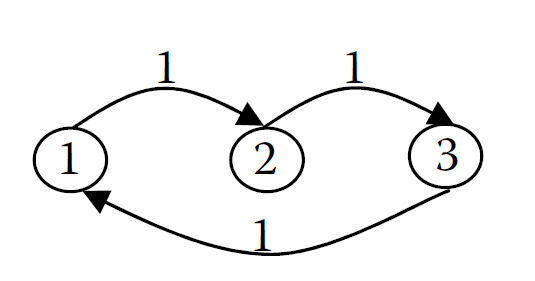
\includegraphics[width=0.5\textwidth]{period.jpg}
        \caption{����Ϊ3�������Ʒ���}
    \end{figure}
\end{itemize}

\indent ���ڻص�����ǰ�������3�����⡣�����ܹ���ǰ���������Կ϶��ش�Ҳ����$\lim\limits_{n\rightarrow \infty}\bm{P}_{n}$ ���������ֵ$\bm{P}_0$��ѡȡ�޹أ���ת�ƾ���$\bm{A}$Ӧ�������3��������
\begin{enumerate}
  \item $\bm{A}$�������������
  \item $\bm{A}$�����Dz���Լ��
  \item $\bm{A}$�����Ƿ����ڵ�
\end{enumerate}

\indent ��������������һ��ͼ\ref{fig:network}�ܷ�������������������������������һ�������Ƿ�һ�����������Ƿ񣬼�$\bm{A}$���������ת�ƣ�������Ϊ$\bm{A}$�ĵ����еĺ���0�� ����ԭ������Ϊ�ڵ�5û�г������ڵ�5��������ҳ����������ҳ���������ϵ�������ҳ�Ǻܶ�ģ�����������Ҫ��$\bm{A}$�д���������ҳ���н�����������ô�����أ����ǿ��Դ�������ҳ$i$ ��ÿһ����ҳ���������Լ�����һ�����ӣ��Ϳ��Խ��������⡣�پ���Щ������ҳ$i$��ÿ����ҳ��ת�����ʶ���Ϊ$\frac{1}{n}$,�൱�ھ��ȷֲ���
\\\indent ��������һ������$n$��Ԫ�ص���������Ϊ������ҳ��ָ������(indicator vector) $\bm{a}$�����$i$��Ԫ��ȡֵ�ӵ�$i$����ҳ�Ƿ�Ϊ������ҳ����������أ�Ϊ������ҳȡ1������ȡ0�����ⶨ��һ������$n$��Ԫ�صĵ�λ������$\bm{e}$,������˼�������ʽ��Ϊ
\begin{equation}
  \bm{S}\leftarrow \bm{A}+\frac{\bm{a}\bm{e}^T}{n}
\end{equation}

\indent ��ͼ\ref{fig:network}��ת�ƾ����������������ת�ƾ������£�
\\\begin{center}$\bm{S}$=$\begin{pmatrix}
0 & \frac{1}{2} & \frac{1}{2}   &0  &0  &0 \\
\frac{1}{2} & 0 & \frac{1}{2}   &0  &0  &0 \\
0 & 1 & 0 &0  &0  &0 \\
0 & 0 & \frac{1}{3}   &0  &\frac{1}{3}  &\frac{1}{3} \\
\frac{1}{6} & \frac{1}{6} & \frac{1}{6}   &\frac{1}{6}  &\frac{1}{6}  &\frac{1}{6}\\
0 & 0 & 0   &\frac{1}{2}  &\frac{1}{2} &0
\end{pmatrix}$ \end{center}

\indent �����������ҳ����������Ƿ���$\bm{S}$�Ƿ�һ������ڶ��������������أ������׾Ϳ��Ը���񶨡��������ǽ�����һ�����ԾͿ���ͬʱ������������⣬������$\bm{S}$ ����ɲ���Լ�ͷ����ڵľ���

\indent �Ծ���$\bm{S}$�������£�
\begin{equation}
  \bm{G}\leftarrow \alpha \bm{S} + (1-\alpha)\frac{\bm{e}\bm{e}^T}{n}
\end{equation}

\indent ����$\bm{e}$�Ǻ���$n$��Ԫ�صĵ�λ������������$0<\alpha<1$ ,Ҳ���������ӣ�һ��ȡֵ0.85��
\\\indent ������ʽ(3)��(4)���������������ǾͰ�ת�ƾ���$\bm{A}$�����������ġ�����Լ�ġ������ڵ�ת�ƾ���$\bm{G}$���Ᵽ֤��$\lim\limits_{n\rightarrow \infty}\bm{P}_{n}$ ���������ֵ$\bm{P}_0$��ѡȡ�޹ء�
\\\indent ������������ӣ��õ�$\bm{G}$���£�$\alpha=0.85$��:
\begin{center}$\bm{G}$=$\begin{pmatrix}
0.0250 & 0.4500 & 0.4500 & 0.0250 & 0.0250 & 0.0250 \\
0.4500 & 0.0250 & 0.4500 & 0.0250 & 0.0250 & 0.0250\\
0.0250 & 0.8750 & 0.0250 & 0.0250 & 0.0250 & 0.0250\\
0.0250 & 0.0250 & 0.3083 & 0.0250 & 0.3083 & 0.3083\\
0.1667 & 0.1667 & 0.1667 & 0.1667 & 0.1667 & 0.1667\\
0.0250 & 0.0250 & 0.0250 & 0.4500 & 0.4500 & 0.0250\\
\end{pmatrix}$ \end{center}

\indent ������ת�ƾ�������������Ĺ���ȷ����PageRank�㷨����ѧ�ϵĿ����ԣ�Ȼ�����Dz����ģ����DZ������������ʵ����Ľ��ͣ���������ȷ������֮ǰ����ĵ��������⣬��``��ҳ����������Ƿ���ĺ���?''��\\
\indent �������������ζ����������̽��з��������Թ�ʽ(3)��(4)���н��ͣ�
\begin{itemize}
\item {\bf �Թ�ʽ(3)�Ľ���}��\\
���������û����ʵ�``������ҳ''ʱ��������``��һ�����ϵ���''�� ���ǻ����з���������ҳ�����ڵ����û���˵�����з��ʵ���ҳ��Ȼ�������Ȥ�йأ������������Ļ������û���������˵�����з����ĸ���ҳ��ȫ������ġ� ����ѧ������˵�� ���൱���ǰ�ת�ƾ���$\bf{A}$�д���������ҳ�������������е�������������$\frac{{\bf e}}{n}$(����${\bf e}$�����з�����Ϊ$1$ ����������$n$ Ϊ�������ϵ���ҳ����)������ѧ���Ա�����ǹ�ʽ(3)��
\item {\bf �Թ�ʽ(4)�Ľ���}��\\
�������û�����һ����������������ɵģ����Ƕ��ٶ����Լ���``�Ը�'',������ȫ�ܵ�ǰ��ҳ���ޣ������ֻ���������ṩ�����ӡ� �����˵�� ���Ǽٶ������û���ÿһ������һ��С��$1$ �ļ��� $\alpha$���ʵ�ǰ��ҳ���ṩ�����ӣ�ͬʱȴҲ��һ������$1-\alpha$������Щ�������ޣ�������ʻ������ϵ��κ�һ����վ������ѧ���Ա�����ǹ�ʽ(4)��
\end{itemize}

\indent ͨ���Թ�ʽ(3)��(4)����ʵ����Ľ��ͣ����ǵõ��������Ľ��ۣ�{\bf ת�ƾ���$\bm{G}$��������ҳ�����ļ����ṩ����ѧ�ϵĿ��еı�֤�����������Ƶ����̾��ж�Ӧ����ʵӦ�ó�����ǿ��֧��}��

\indent �ѹ�ʽ(4)��$\bm{G}$�ı���ʽ�����ʽ(1)��(2)�е�A,�õ����µ�������ʽ��
\begin{equation}
  \bm{P}=\left[\alpha\left(\bm{A}^T+\frac{\bm{e}\bm{a}^T}{n}\right)+(1-\alpha)\frac{\bm{e}\bm{e}^T}{n}\right]\bm{P}
\end{equation}
\begin{equation}
  \begin{split}
    \bm{P}_{n+1}=\left[\alpha\left(\bm{A}^T+\frac{\bm{e}\bm{a}^T}{n}\right)+(1-\alpha)\frac{\bm{e}\bm{e}^T}{n}\right]\bm{P}_n,n=0,1,\cdots,\infty,\mathrm{given}~ \bm{P}_0
  \end{split}
\end{equation}
\indent ����һ��֮�󣬰�������ǰ���Ψһ���⣬��������ˣ�����ģ�ȷ����ʽ(5)��$\bm{P}$������֮�ȼ۵Ĺ�ʽ(6)��$\lim\limits_{n\rightarrow \infty}\bm{P}_{n}$��

\indent ���ݵ����������㷨�ܼ򵥣����Ը��������PageRank��ʼֵ��ÿ��������PageRankֵ���������Σ���PageRankֵ���������仯������������ʱ�������㷨������������㷨�Ľ��������Dz�ֵ������һ�׷���С��һ��Ԥ�趨����ֵ$\epsilon$��ͽ����㷨������

  \begin{algorithm}[htb]
  \caption{PageRank-Iterate(G).}
  \begin{algorithmic}[1]
    \STATE $P_0\leftarrow \bm{e}/n$
    \STATE $k\leftarrow 1$
    \REPEAT
    \STATE $\bm{P}_{k+1}=\left[\alpha\left(\bm{A}^T+\frac{\bm{e}\bm{a}^T}{n}\right)+(1-\alpha)\frac{\bm{e}\bm{e}^T}{n}\right]\bm{P}_k$
    \STATE $k\leftarrow k+1$
    \UNTIL $\parallel\negthickspace P_k-P_{k+1}\negthickspace\parallel_1<\epsilon$
    \RETURN $P_k$
  \end{algorithmic}
\end{algorithm}

\indent ��ʽ(6),��$\bm{P}_{k+1}=\bm{G}\bm{P}_k$��ƽ�ȷֲ�(��PageRankֵ)��ת�Ƹ��ʾ���$\bm{G}$���������ֵ$(=1)$����Ӧ����������,���Ծ����Ŷ��������ԣ�������������������ֵ�ķ���ȡ�����������$\alpha$ֵ����$1$������$\bm{G}$�Ĵ�����ֵ����֮����$1$���Ӷ�����PageRank��$\alpha$ֵ��ѡ�������������������������㷨�������ٶȻή�͡�Ҳ����˵����������$\alpha$ԽС�������ٶ�Խ�졣��$\alpha$Ҳ����̫С�� ��Ϊ̫С�Ļ���``PageRank''������IJ��֣� ������ҳ��ı˴�����Ϊ����������˼·�ͱ������� (��Ϊ�ⲿ�ֵĹ���������$\alpha$)�� ����Ȼ�ǵò���ʧ�ġ� ��ˣ� ��$\alpha$��ѡȡ���кܶ����ԵĿ���Ҫ���� ����Ͳ�������ѡ�����ֵ�� �� = 0.85��
\section{PageRank����չ��Timed-PageRank}
�������ϵ�����ҳ�������ӣ�ͬʱ���ϵ��оɵ���ҳ��ù�ʱ��Ȼ����Щ�ɵ���ҳ�ܶ඼����ɾ�����������������鷳����Ϊ��Щ��ʱ����ҳ�����ڹ�ȥ�ij�ʱ��������˴��������Ӷ�����ܸߣ�����Щ��������Ϣ�ĸ�������ҳ��ȴ��Ϊû���㹻������������ƫ�͡�
\\\indent Ϊ��Ӧ�����������Timed-PageRank�㷨��PageRank�㷨������������һ��ʱ��ά�ȣ�����˼����ʵ�ܼ򵥣���������Ȼ������PageRank����������������Ʒ���ģ�ͣ���֮ͬ������Timed-PageRank�������ó�����������$\alpha$����������һ��ʱ��ݼ�����$f(t)(0\leq f(t)\leq 1)$��``�ͷ�''��ʱ����ҳ���˴���t��ָ��ǰʱ�����ҳ�ϴθ���ʱ��IJ�ֵ��������$f(t)$������Ϊ�����ҳ�����ӵĸ��ʣ�$1-f(t)$���Dz�������ҳ�ϵ����Ӷ�ֱ������һ�����ѡ����ⲿ��ҳ�ĸ��ʡ���ô����һ���ض�����ҳ$i$��������ѡ��
\begin{itemize}
  \item ��$f(t)$�ĸ������ѡ��һ������������
  \item ��$1-f(t)$�ĸ��ʲ�ͨ����������ij�������ҳ��
\end{itemize}

\section{Perron�CFrobenius ����}
\indent ��$\bm{A}=\left(a_{ij}\right)$Ϊһ��$n\times n$��������$\forall 1\leq i,j\leq n,a_{ij}>0$����þ������������ʣ�
\begin{enumerate}
  \item $\bm{A}$����һ����ʵ��������ֵ$\lambda^{*}$������Perron������Perron�CFrobenius����ֵ��ʹ��������������ֵ(������������ֵ)��ģ������С��
  \item $\lambda^{*}$ֻ��Ӧһ����������$\bm{v}$��
  \item $\lambda^{*}$����Ӧ����������$\bm{v}$������Ԫ�ض�Ϊ��ʵ����
  \item $\lambda^{*}$�������������ֵ����Ӧ������������Ԫ��������һ��Ϊ����������
  \item $\lim_{k \rightarrow \infty} \frac{\bm{A}^k\bm{e}}{{\lambda^{*}}^k}= \bm{v}$
  \item $\min\limits_i \sum\limits_{j} a_{ij} \le \lambda^{*} \le \max\limits_i \sum\limits_{j} a_{ij}$
\end{enumerate}
\begin{thebibliography}{9}
\bibitem{}{¬����},{�ȸ豳�����ѧ}, \url{http://www.changhai.org/articles/technology/misc/google_math.php}, 12/05 2010.
\bibitem{}{����Դ,л����},{��ѧ��ģ����ѡ��}.
\bibitem{}{Cannel\_2020},{Google�����������}, \url{http://blog.csdn.net/cannel_2020/article/details/7672042}, 06/18 2012.
\bibitem{}{�װ뾶}, \url{http://zh.wikipedia.org/wiki/%E8%B0%B1%E5%8D%8A%E5%BE%84}.
\bibitem{}{����������Ӧ�ã�PageRank�㷨Google��������İ���}, \url{http://f.dataguru.cn/thread-330418-1-1.html}, 07/20 2014.
\bibitem{}{�������ǻ����Ż�������� Google PageRank�㷨}, \url{http://chaxin.gdinfo.net/web/www/dialog/index.php/Dialog/%E7%B3%BB%E7%BB%9F%E6%A6%82%E8%BF%B0/%E7%B3%BB%E7%BB%9F%E6%A6%82%E8%BF%B0ch5_5.htm}.
\bibitem{}{����Դ},{��ѧģ�ͣ�������}
\bibitem{}{Perron�CFrobenius theorem}, \url{http://www.cnblogs.com/ZhangShuo/articles/1866748.html }, 10/24 2013.
\bibitem{}{Xindongwu, Vipin Kumar},{Top 10 Algorithms in Data Mining. ICDM 2006 Panel 12/21/2006}
\bibitem{}{We Recommend a Singular Value Decomposition}, \url{http://www.ams.org/samplings/feature-column/fcarc-svd }.
\bibitem{}{ccjou},{�����Q��ꇿ��������ǻ����C��}, \url{https://ccjou.wordpress.com/2011/02/09/%E5%AF%A6%E5%B0%8D%E7%A8%B1%E7%9F%A9%E9%99%A3%E5%8F%AF%E6%AD%A3%E4%BA%A4%E5%B0%8D%E8%A7%92%E5%8C%96%E7%9A%84%E8%AD%89%E6%98%8E/}, 02/09 2011.
\bibitem{}{iMetaSearch},{Latent Semantic Analysis (LSA) Tutorial },    \url{http://www.puffinwarellc.com/index.php/news-and-articles/articles/33-latent-semantic-analysis-tutorial.html?start=6}.
\end{thebibliography}

\end{document}
